\chapter{State of the Art}

This state-of-the-art section investigates the emerging status of real-time data communication in modern data systems. It examines three interrelated domains viz- WebTransport streams, Kubernetes and its support for emerging web protocols, and modern streaming platforms. WebTransport \cite{webtransport-draft} built on top of the QUIC transport protocol \cite{rfc9000} and HTTP/3 \cite{rfc9114} introduces new features which enables low-latency, bidirectional communication over the internet. Its ability to support both reliable and unreliable data transfers makes it suitable for latency-sensitive applications such as live video streaming. By avoiding head-of-line blocking and supporting QUIC enabled features such as connection migration, WebTransport addresses several limitations existed in other technologies like HTTP/2, positioning itself as a next-generation protocol for web applications.


In conjunction, we will look at Kubernetes \cite{kubernetes-docs}, which is one of the most widely used systems for container orchestration, which can handle large applications deployed across different machines. Additional support for newer generation protocols like QUIC, HTTP/3, and WebTransport in Kubernetes brings its own set of challenges while we explore the state-of-the-art solutions. This also covers several tools and components and their explanations, providing better context. Several Ingress solutions, the Gateway API, and QUIC library implementations are explored. Finally, we investigate the web streaming use case and technologies that work together to support real-time systems to process big data.




\section{Networking Concepts}
\subsection{OSI Model}
The Open Systems Interconnection (OSI) Model \cite{kurose2017} essentially breaks down communication networks into 7 layers, viz., Physical, Data Link, Network, Transport, Session, Presentation, and Application Layer. Each of these layers handles specific tasks and abstracts its functionality from the other layers. The physical layer is responsible for moving raw bits wired using cables or wireless using links. The data link layer deals with the management of data and ensures it is error-free as it travels to other devices. The network layer is responsible for handling routing decisions and deals with the transmission and reception of messages. The session, presentation, and application layers deal with managing sessions, formatting data, and running and creating application-formatted data. It's where the application services run. With respect to our dissertation topic, QUIC is a transport layer protocol, whereas HTTP/3 and WebTransport are application layer protocols.


\subsection{IP Frames}
Internet Protocol (IP) Frames, also called Packets, are a protocol structure that operates at the networking layer, which encapsulates the data. In its structure there are source and destination IP addresses, which are responsible for inter-network routing. An IP packet consists of a header that contains the IP address and protocol type, and a payload which contains the data from the underlying protocol that was used. IP packets are most critical for routing TCP, UDP, or QUIC transport data across the internet.

\subsection{Network Interface}
Network interfaces operate between the Physical and Data Link layers,. It acts as an interface between the hardware and software for network communication. Examples are Ethernet Network Interface Cards (NICs) (e.g., eth0) and wireless adapters (e.g., wlan0), which is responsible for converting raw bits to signals and for processing Ethernet frames. Any form of communication passes through a network interface. Heres a snapshot of some network interfaces on my device.
Note that we have an Maximum Transmission Unit (MTU) parameter equal to 1500.

\begin{figure}[h]
\caption{Network Interfaces}
\centering
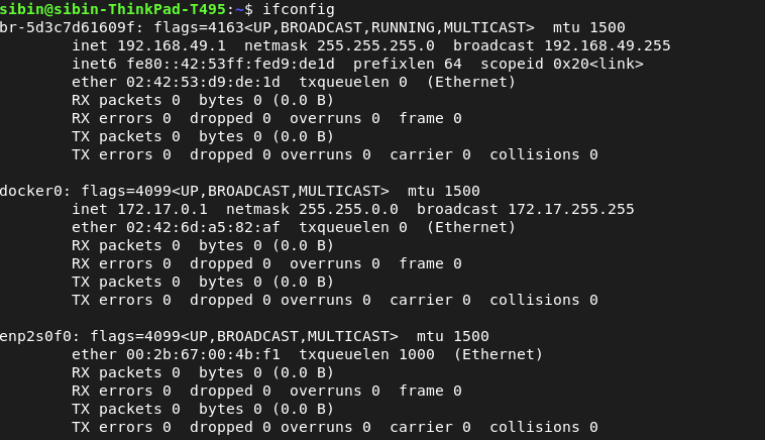
\includegraphics[width=1\textwidth]{SOA/NIC.png}
\end{figure}

\subsection{MTU (Maximum Transmission Unit)}

The MTU decides the maximum packet size that can be transmitted over a network without being subject to fragmentation (splitting of packets). In the images above it is seen that all the network interfaces have an MTU of 1500 Bytes. In order to work with larger sized data, modiications to the protocols MTU must be done to accomadate the changes




\subsection{Packets}

Packets are bundled units of data that is transmitted across network interfaces. It is idenitified as: bits  for Physical Layer, frames for Data Link, packets for Network, and segments or datagrams for Transport Layer. For HTTP/3 App data, Ethernet frames encapsulates IP packets which contain UDP datagrams which carry QUIC Pakcets with multiple streams enabling multiplexing.

\begin{figure}[H]
\caption{Flow of Packets}
\centering
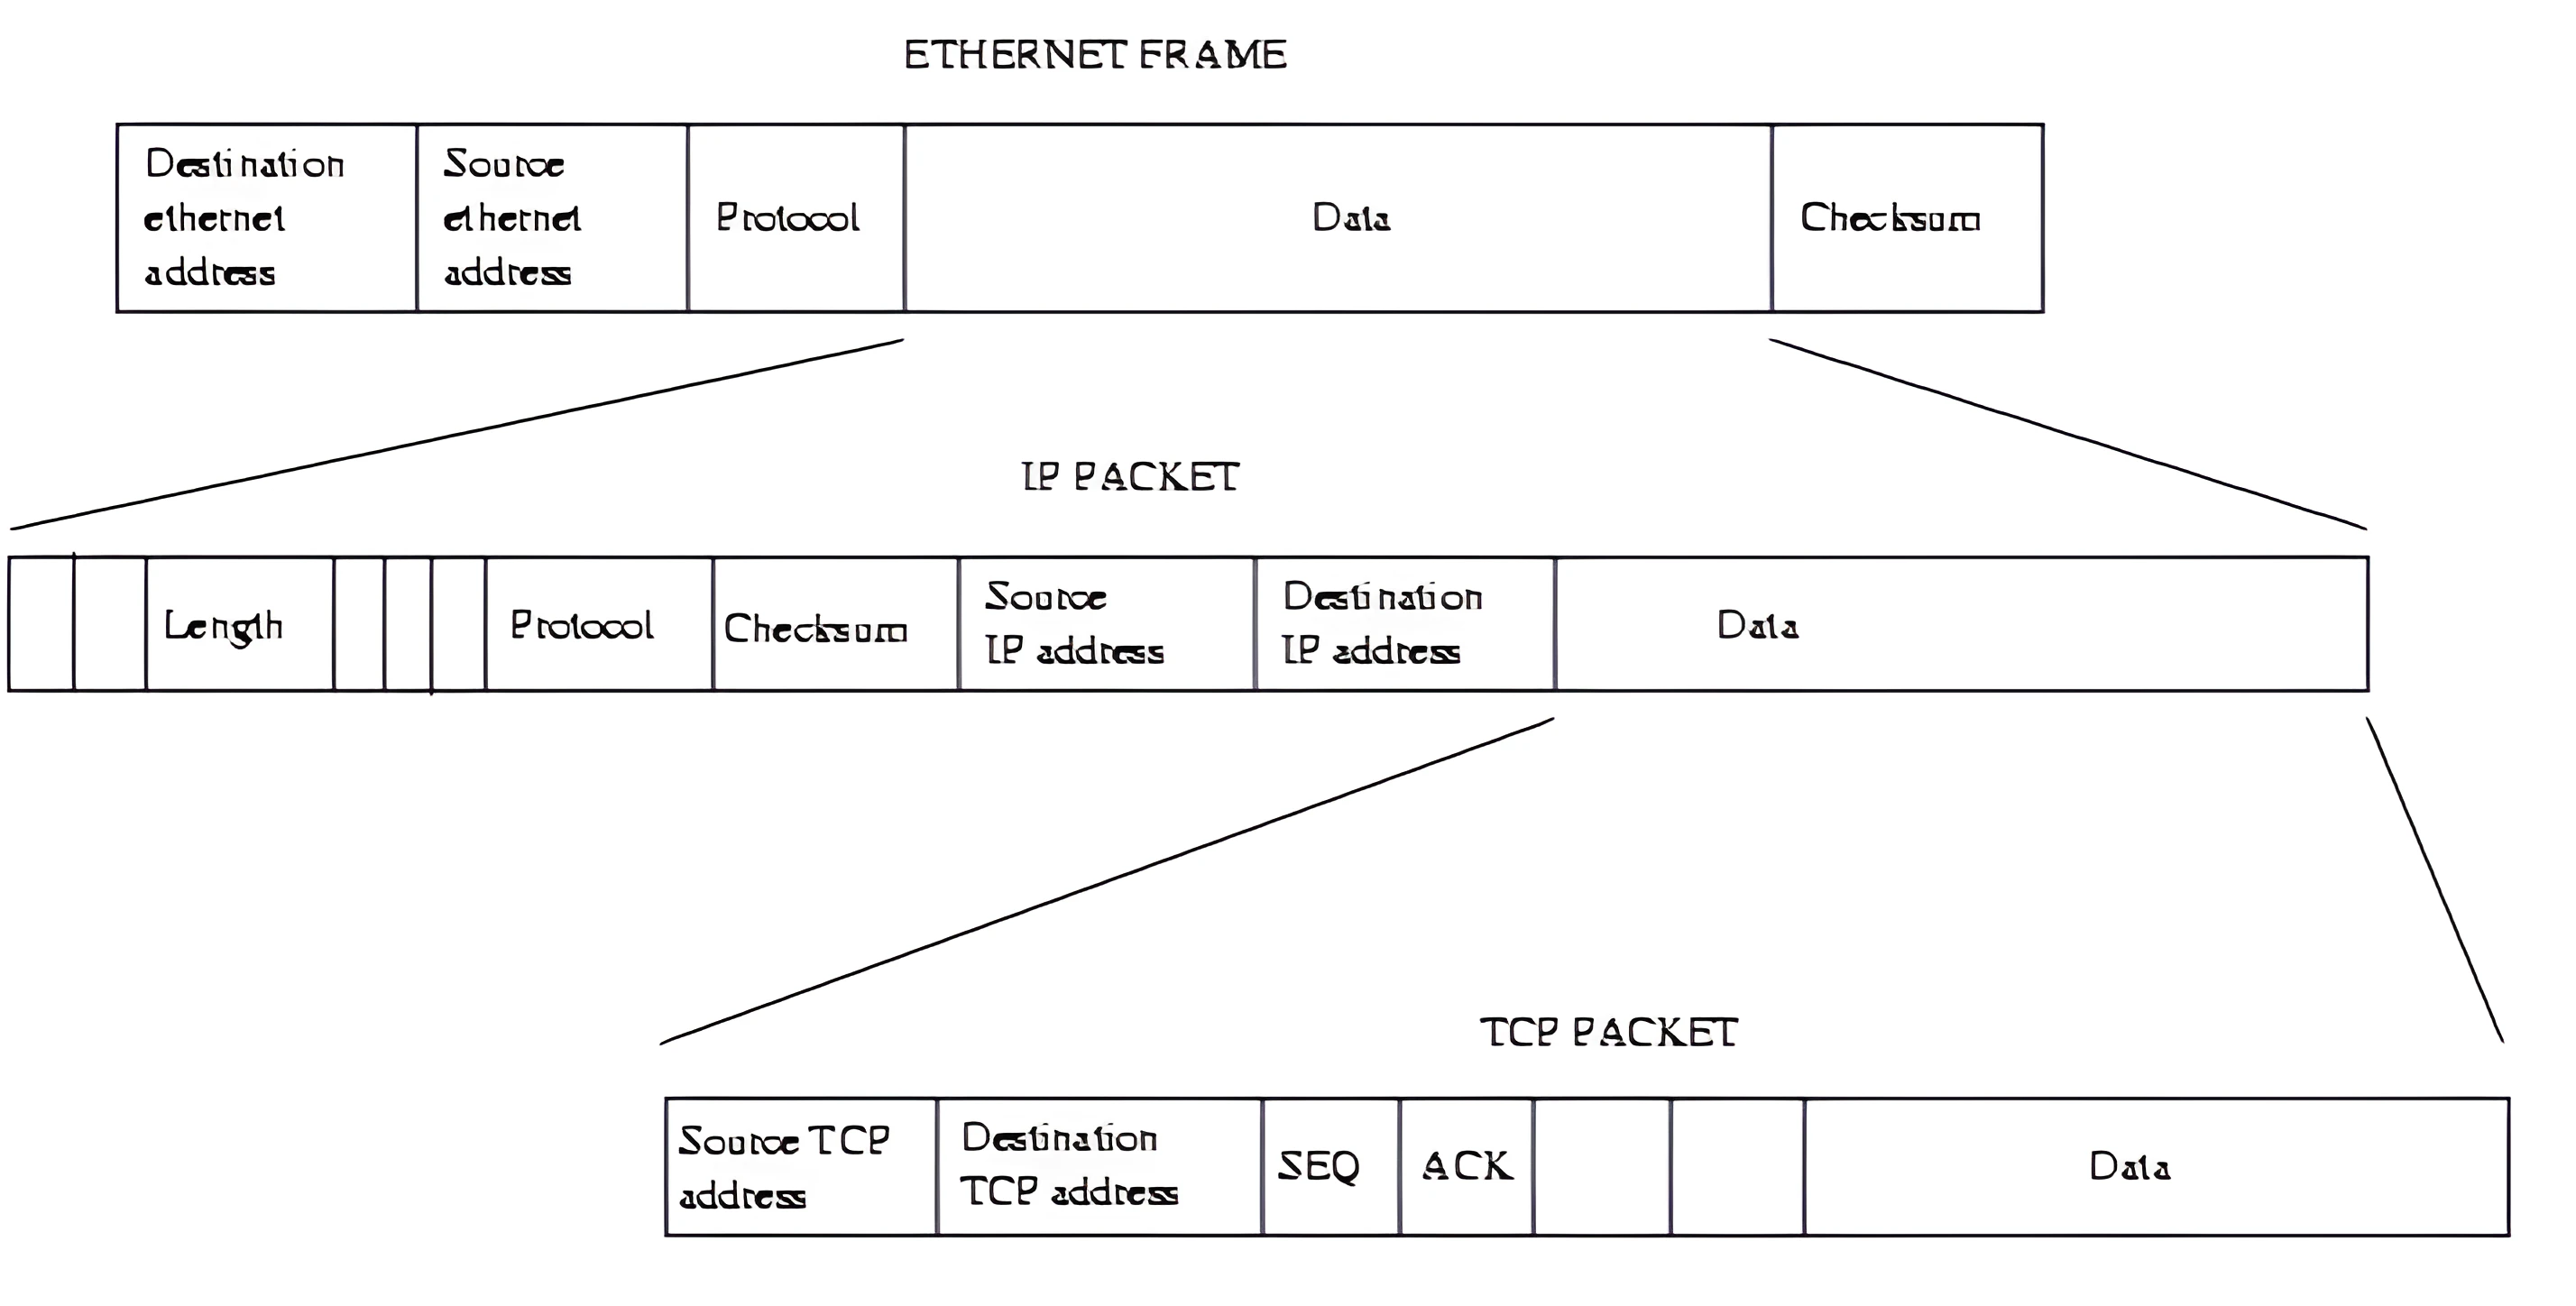
\includegraphics[width=1\textwidth]{SOA/packets.png}
\end{figure}

\subsection{TCP (Transmission Control Protocol)}


TCP is a connection oriented protcol which ensures data reliability with several mechanisms such as Acknowledgments (Acks), Retransmissions and in-order delivery \cite{kurose2017}. TCP fucntions by establishing a three-way handshake between client and server. The handshakes can be seen in the figure below. TCP requires roundtrups to initiate communication and when it works with higher level application protocols which require TLS, it impacts performance introducing latency particularly during the connection setup.


\begin{figure}[H]
\caption{TCP Handshake}
\centering
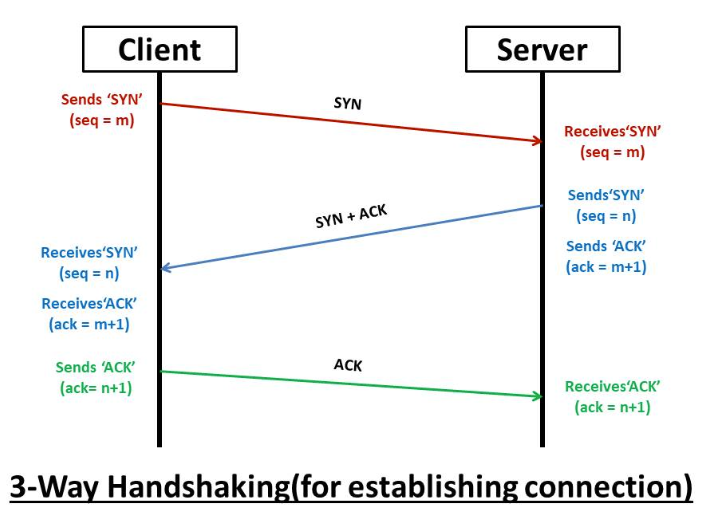
\includegraphics[width=0.7\textwidth]{SOA/tcp.png}
\end{figure}


TCP's design introduced challenges such as Head of Line Blocking. This is an issue which impacts performance for applications at scale. This HoL problem basically means that when a packet is lost, all subsequent packets are waited until the packet reaches the destination. Several approaches are followed to mitigate this issue such one such approach is multi-path TCP where data is sent over multiple paths avoiding this issue but the underlying protocol still suffers from this issue and the middlebox configuration is a concern.

TCP guarantees reliability making it ideal for application which require stringent ordered delivery. However, due to middle box configurations and TCPs reliance on outdated implementations restricts it from being highly performative.


\subsubsection{Operating System (OS) Configurations for TCP}

In linux machines, TCP's state is exposed  through the /proc/next/tcp path which is a virtual filesystem part of the procfs interface. This provides dynamically generated real time information about the active TCP connections which includes local addresses, remote addresses, port numbers, connection states and sequence number. Each entry persists for 60s  in the TIME\_WAIT state. (Protocol Compliance Requirement). The confgurations for handling concurrent tcp connections are monitored via parameters such as tcp\_max\_orphans, fs.file-max, and ulimit -n. Modification to these parameter increases the set limits to increase performance. 


\subsubsection{TCP Congestion and Flow Control}

TCP’s congestion control is managed by the sender with the congestion window ('cwnd'), its initialized with a small value at the start (e.g., 10 segments) and adjusted based on network feedback from the server. During the slow start phase, 'cwnd' grows exponentially with reception of acknowledgments (ACKs), when a packet loss is detected via duplicate ACKs or timeouts, it triggers a reduction in 'cwnd' to mitigate network congestion with the help of flow control which is managed by the receiver’s advertised window ('rwnd'), it prevents buffer overflow by limiting the sender’s transmission rate.





\subsection{Middle-Box Ossification}
Middleboxes become bottlenecks because of its old implementation and inability to update widely adopted middleboxes. In context of tcp it means the network devices like firewalls, routers have tcp implementation at their kernel level, which becomes an issue when updates to the core implementation of protocol are required.


\subsection{UDP}

User Datagram Protocol (UDP), is a connectionless protocol that focuses low latency than reliability \cite{kurose2017}. This is due to the fact that it lacks the built-in mechanisms for retransmission, ordering, or congestion control and hence makes it suitable for applications where speed is critical, and occasional packet loss is tolerated. Due to this it enables one-RTT communication which is ideal for Domain Name System (DNS) queries and real-time media streaming like online gaming, video streaming, etc. But, its lack of reliability, security, and congestion control makes it unsuitable for use in cases requiring guaranteed delivery.

\subsubsection{UDP Packet Structure}

UDP operates within a simple packet structure encapsulated as follows:

\begin{itemize}
    \item \textbf{Ethernet Frame}: It contains the Media Access Control (MAC) addresses(source and destination) and the control information for physical transmission.
    \item \textbf{IP Packet}: It encapsulates the source and destination IP addresses for routing.
    \item \textbf{UDP Datagram}: It includes the source and destination ports and the data(payload), with no reliability or ordering mechanisms.
\end{itemize}

UDP’s minimalist design enables low-latency communication but it lacks the robust features of TCP, and hence it requires application-level handling of reliability and ordering where needed.

UDP, lacking connection state, does not maintain persistent entries in /proc(the virtual filesystem used to expose kernel and process information). Both protocols face challenges with middleboxes(see section 2.1.7), such as firewalls, which often rely on outdated TCP configurations, complicating updates for advanced features like TCP Fast Open.

\subsection{Limitations of Traditional Transport Layer Protocols}

The foundational transport protocols of the internet, TCP and UDP, face well-documented limitations that hinder performance, scalability, and adaptability in modern network environments.

TCP suffers mostly from \textit{head-of-line (HOL) blocking}, a condition where the loss of a single packet holds up the delivery of all subsequent packets in that stream, thereby leading to increase in latency and degrading user experience. In addition to internal limitations, TCP evolution is impeded by \textit{middlebox ossification} see section 2.1.7. Network devices like legacy firewalls and Network Address Translation (NAT) gateways often do not recognize newer TCP features, such as, TCP Fast Open or Multipath TCP, blocking their deployment and stalling protocol innovation across the wider internet.

On the other hand, UDP, designed as a minimal transport layer, circumvents many of TCP’s internal restrictions but introduces its own set of challenges. It lacks built-in mechanisms for reliability, packet ordering, and congestion control, forcing developers to reimplement these features at the application level. Moreover, UDP is susceptible to \textit{NAT rebinding}, where NAT devices revoke and reassign port mappings after idle periods, leading to unexpected connection drops.

Both TCP and UDP also has  host-level limitations. Important among these is the finite ephemeral port range, typically around 65,000 ports per IP address which restricts the number of simultaneous connections to the same destination. In high-throughput systems, the availability of file descriptors and system memory further limits the scale of concurrent network connections, imposing additional resource constraints.

These protocol-level and systemic challenges have led to the development of next-generation transport protocols like QUIC, that aim to address these shortcomings in a modern, application-aware manner.

\subsection{QUIC Protocol}

The Quick UDP Internet Connections (QUIC) protocol represents an innovative transport layer solution designed to address the limitations of traditional TCP-based protocols, particularly in the context of modern web applications. Unlike TCP, which relies on sequential TLS and TCP handshakes, QUIC leverages UDP to combine transport and security handshakes into a single step, significantly reducing connection setup latency.

QUIC’s design aims to provide TCP-like reliability, stream multiplexing, and congestion control (see section 2.1.10.2) while mitigating TCP’s drawbacks, such as HOL blocking and the need for kernel-level updates across network infrastructure. By operating over UDP, QUIC enables deployment without requiring modifications to middleboxes like firewalls or routers, which often struggle with outdated TCP configurations. 

QUIC is a transport protocol that integrates the TLS 1.3 handshake with its initial transport handshake, achieving connection setup in a single RTT. QUIC also incorporates reliability, in-order delivery, and congestion control, addressing UDP’s limitations while retaining its low-latency characteristics. The protocol supports multiplexing through independent streams within a single connection, eliminating inter-stream HOL blocking, a significant issue in TCP-based HTTP/2. 

\subsubsection{QUIC Packet Structure}

QUIC operates within a layered architecture, encapsulated as follows:

\begin{itemize}
    \item \textbf{Ethernet Frame}: Contains MAC addresses and control information for physical transmission.
    \item \textbf{IP Packet}: Encapsulates source and destination IP addresses for network routing.
    \item \textbf{UDP Datagram}: Provides a lightweight, connectionless transport layer for QUIC packets.
    \item \textbf{QUIC Packet}: Includes a header (e.g., Short Header with Destination Connection ID and Packet Number) and an encrypted payload containing frames such as ACK, STREAM, and datagram frames.
\end{itemize}

\begin{figure}[H]
\caption{QUIC vs TCP packet Structure}
\centering
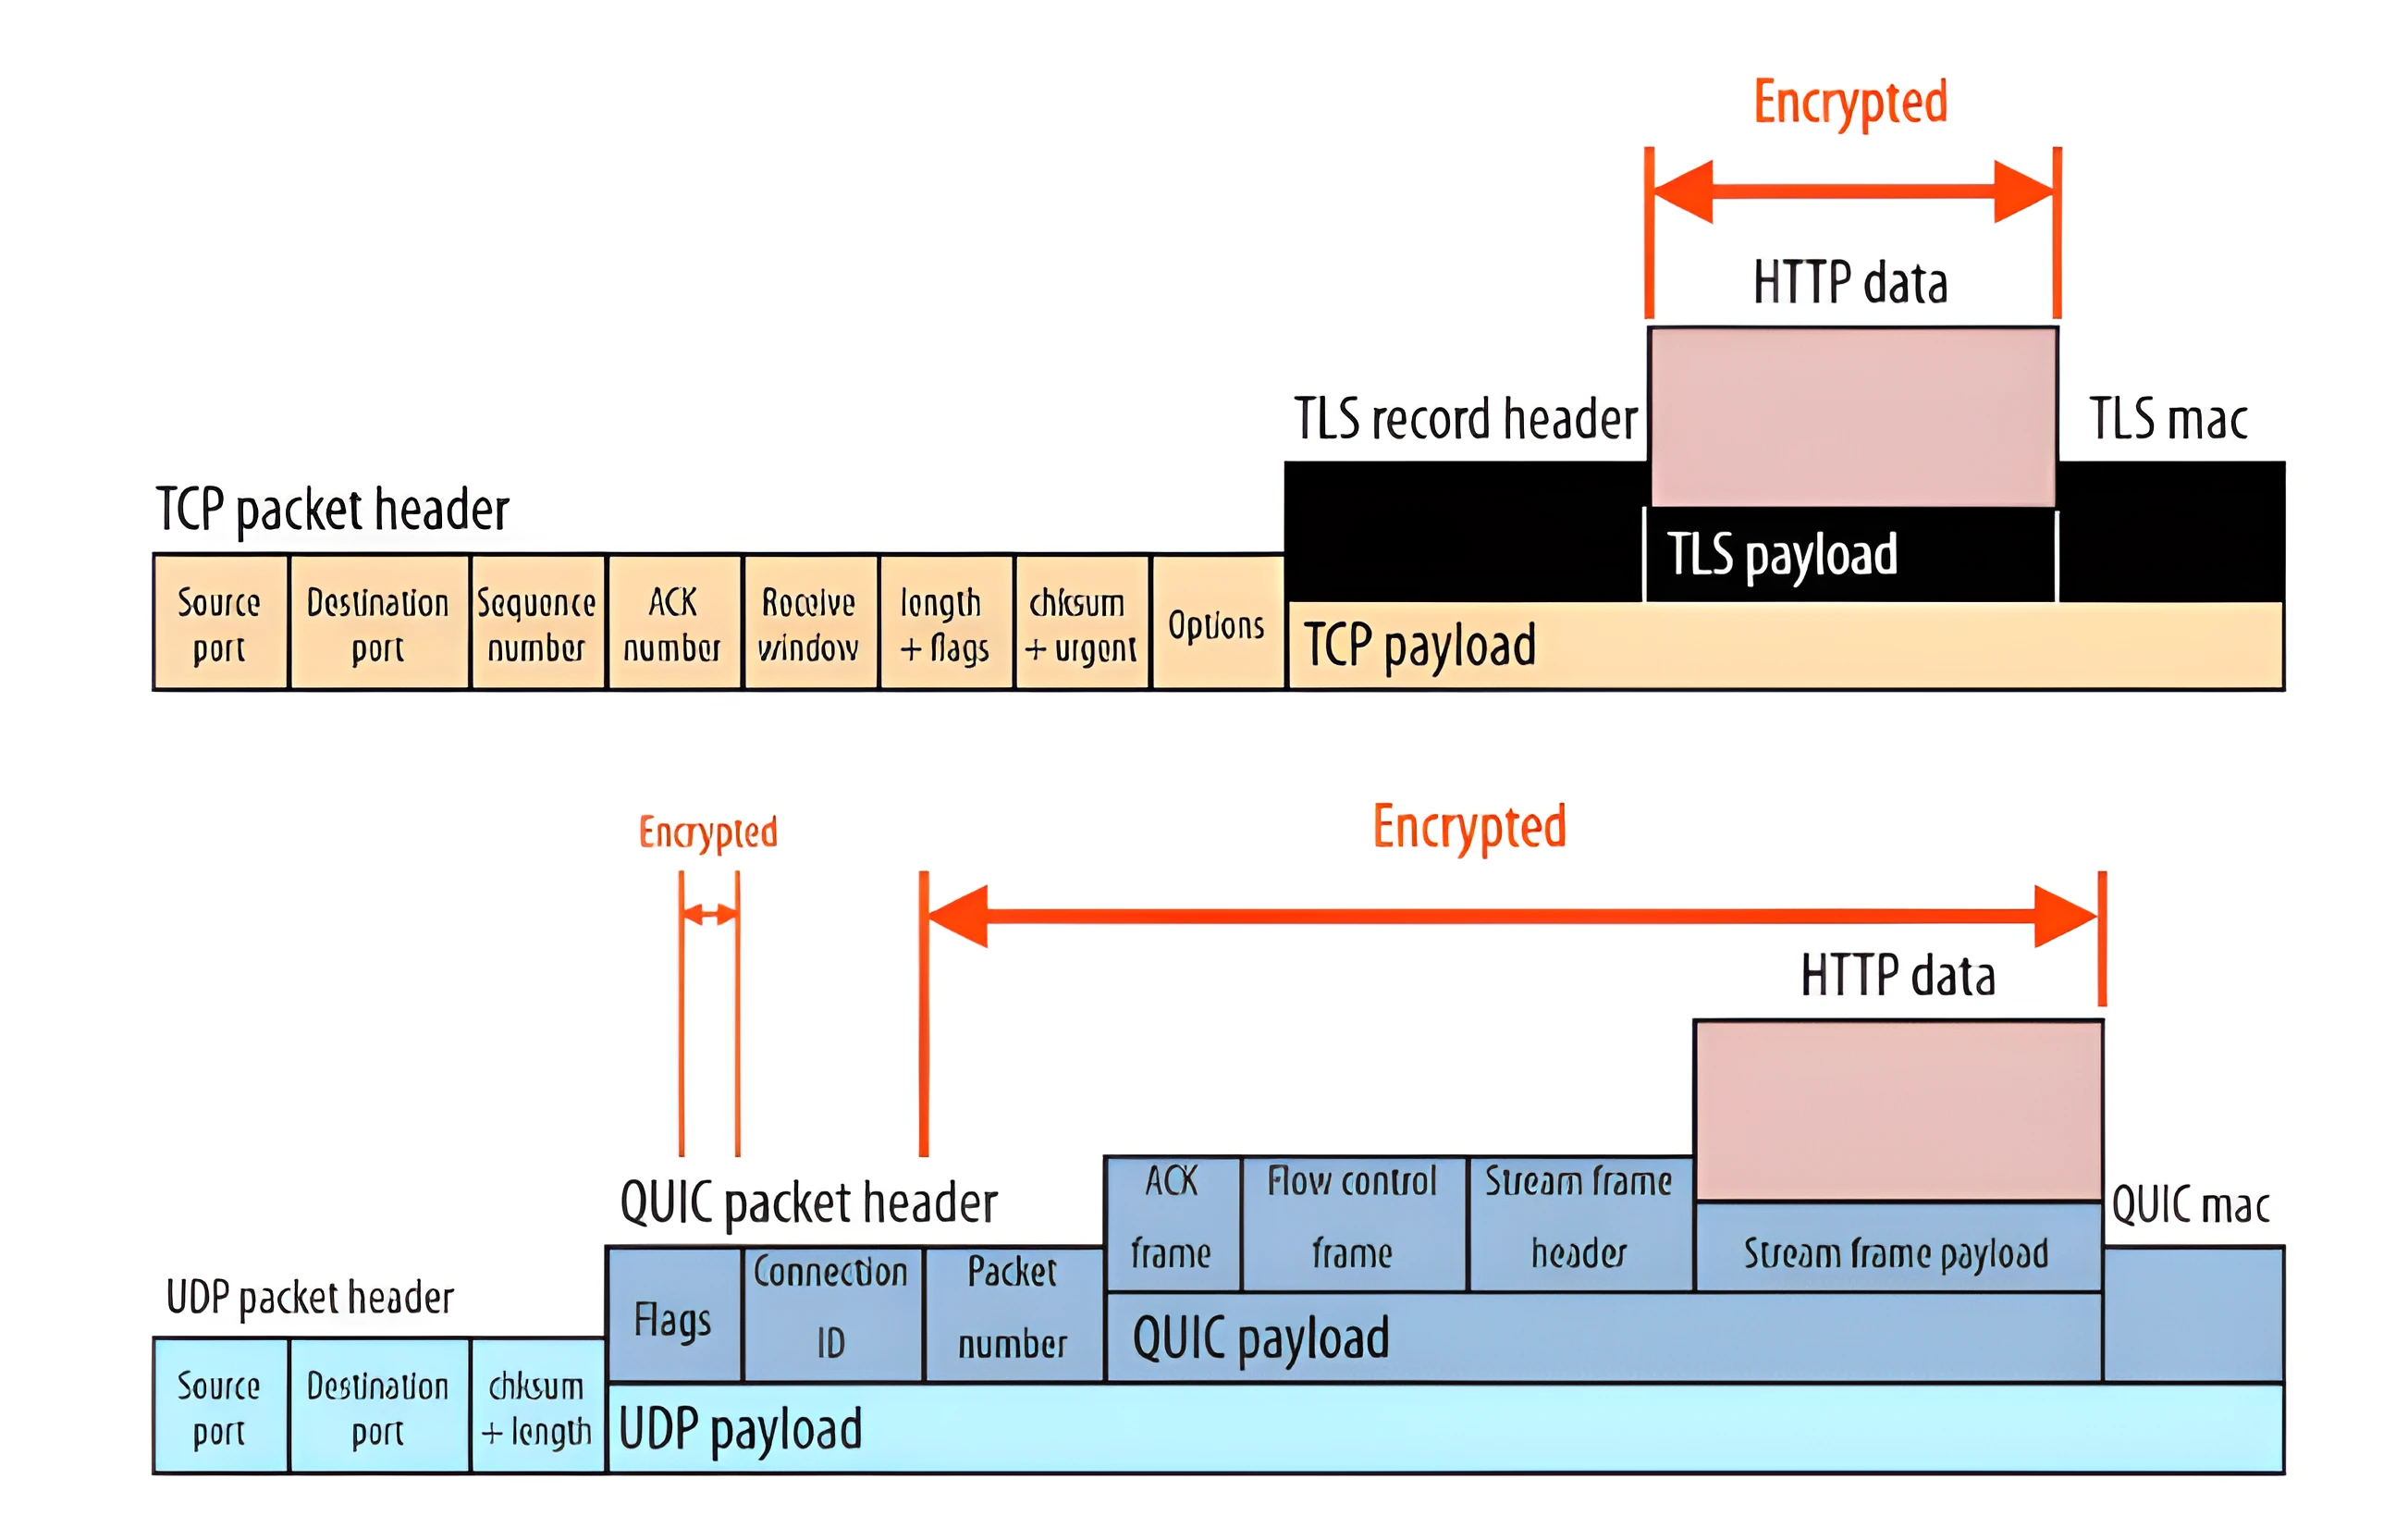
\includegraphics[width=1\textwidth]{SOA/quicntcp.png}
\end{figure}


For example, in above figure \cite{marx2021-http3} depicting QUIC Packet structure we can see that quic packets are sent as a udp packet in its payload


\subsubsection{Congestion and Flow Control}

QUIC implements congestion control at the connection level, using a sender-managed congestion window (\texttt{cwnd}) that adjusts based on network conditions, similar to TCP. The sender initializes \texttt{cwnd} conservatively (e.g., 10 segments) and increases it exponentially during the slow-start phase or linearly during congestion avoidance, reducing it upon detecting packet loss. Flow control, managed by the receiver’s advertised window (\texttt{rwnd}), operates at the stream level, ensuring that senders do not overwhelm receiver buffers.

Stream prioritization, supported by QUIC’s APIs, allows developers to assign higher priority to critical streams (e.g., audio over video), optimizing resource allocation. Frame coalescing further enhances efficiency by packing multiple frame types into a single UDP datagram, following the Maximum Transmission Unit (MTU).

\subsubsection{Implementation Considerations}

QUIC’s user-space implementation, unlike TCP’s kernel-space design, enables rapid iteration but introduces performance overhead. Debugging tools like \texttt{qlog} and \texttt{qvis} facilitate debugging and analysis of QUIC’s advanced features, such as multiplexing and congestion control. For large file downloads, QUIC supports range-based requests which is similar to HTTP Range headers, allowing recovery of broken connections by requesting only missing byte ranges, provided servers support partial content requests.

QUIC’s ability to multiplex streams and datagrams within a single connection enhances its suitability for applications requiring concurrent data transfers, such as web browsing and file downloads. However, intra-stream HOL blocking persists, as data within a single stream is delivered in order, requiring retransmission of lost packets before subsequent data can be processed. In this dissertation implementation, we will be focusing on the feature multiplexing (multiple independent streams per connection).

\subsection{Comparison of TCP, UDP, and QUIC}

The following table summarizes the key features of QUIC compared to TCP and UDP, highlighting its hybrid design:

\begin{table}[H]
\centering
\begin{tabular}{|p{4cm}|c|c|c|}
\hline
\textbf{Feature} & \textbf{UDP} & \textbf{TCP} & \textbf{QUIC} \\
\hline
Connectionless & Yes & No & Yes (UDP-based) \\
\hline
Reliable Delivery & No & Yes & Yes \\
\hline
In-Order Delivery & No & Yes & Yes (per stream) \\
\hline
Multiplexing & No & No & Yes (multiple streams per connection) \\
\hline
Built-in TLS & No & No (external TLS) & Yes (TLS 1.3 mandatory) \\
\hline
Head-of-Line Blocking & No & Yes (affected) & No (avoids inter-stream blocking) \\
\hline
Connection Migration & No & No & Yes (survives IP changes) \\
\hline
\end{tabular}
\caption{Comparison of features across UDP, TCP, and QUIC}
\label{tab:tcp-udp-quic-comparison}
\end{table}



\section{HTTP Protocols}

The HyperText Transfer Protocol (HTTP) has undergone multiple changes since its inception, which helped it evolve in order to meet the growing demands of modern web applications. Each version introduces significant changes in how data is structured, delivered, and optimized over networks.

\subsection{HTTP/0.9}

Introduced in 1991, HTTP/0.9 was the earliest version of the protocol, designed for the simple retrieval of HTML documents. It supported only the \texttt{GET} method, and responses consisted of raw HTML without headers. Lacking support for metadata, status codes, or content types, HTTP/0.9 was limited to extremely basic use cases. It operated over a single TCP connection and closed the connection immediately after the response, making it inefficient for handling multiple resources.

\subsection{HTTP/1.1}

Standardized in 1997 (RFC 2068, later updated by RFC 2616 and RFC 7230 series), HTTP/1.1 allowed multiple requests and responses to be sent over a single TCP connection hence introducing persistent connections \cite{kurose2017}. It added  methods like \texttt{PUT}, \texttt{DELETE}, and \texttt{OPTIONS} and support for chunked transfers, caching mechanisms, virtual hosting. However, HTTP/1.1 had head-of-line blocking at the application layer which severely limit performance, particularly for resource-heavy web pages due to fundamentally being constrained by the serialized nature of TCP streams.

\subsection{HTTP/2}

HTTP/2 was published in 2015 (RFC 7540), in order to fix the performance limitations of HTTP/1.1 \cite{kurose2017}. It introduced binary framing, header compression (HPACK), and multiplexing, allowing multiple concurrent streams over a single TCP connection. These changes led to significant reduction in latency and improved page load times. As HTTP/2 still has underlying TCP, it remains susceptible to TCP-level head-of-line blocking. If a packet is lost, the entire TCP connection stalls until retransmission is complete, affecting all multiplexed streams.

\subsection{HTTP/3}

HTTP/3 is an application-layer protocol built on top of QUIC, developed to overcome the limitations of HTTP/2, particularly head-of-line (HOL) blocking caused by its reliance on TCP \cite{rfc9114} \cite{marx2021-http3}. By replacing TCP with QUIC (which runs over UDP), HTTP/3 introduces features such as built-in encryption (TLS 1.3), reduced handshake latency, connection migration, and robust stream multiplexing. These capabilities make HTTP/3 ideal for modern web environments, including mobile-first, real-time, and high-throughput applications.

\subsubsection{Multiplexing, Flow Control, and Congestion Handling}

HTTP/3 benefits directly from QUIC’s architecture, which provides independent, multiplexed streams within a single connection. This means that packet loss on one stream doesn’t block others, resolving the HOL blocking issue thats present in TCP. It allows more efficient and smoother data delivery, especially over unreliable or variable networks.

QUIC also implements stream-level flow control, ensuring that each stream can progress without interfering with others. Additionally, it features advanced congestion control algorithms (e.g., BBR or CUBIC), similar to TCP, but designed to react faster and recover more effectively in poor network conditions. These mechanisms enable HTTP/3 to maintain low latency and high performance across diverse network environments.

HTTP/3, through QUIC, provides several key enhancements including faster connection establishment via reduced round trips, encryption by default using TLS 1.3, stream multiplexing without HOL blocking, connection migration in case of IP changes (e.g., switching from Wi-Fi to mobile data), and 0-RTT support allowing faster repeat connections.


\subsubsection{Implementation and Adoption}

HTTP/3 is supported by major implementations such as Google’s quiche, Cloudflare’s quiche, Mozilla’s neqo, and Facebook’s mvfst, with integration into popular web servers like nginx, LiteSpeed, and Apache. Browser support is strong, with Chrome, Firefox, Safari, and Edge already implementing HTTP/3.

However, widespread adoption is still in progress. Challenges such as middlebox compatibility, UDP tuning limitations, and infrastructure readiness hinders deployment. Nonetheless, as HTTP/3 continues to demonstrate tangible performance and reliability improvements, especially in mobile and high-latency scenarios, its adoption is steadily accelerating.


\subsection{Summary Table: HTTP Protocol Evolution}

\begin{table}[H]
\centering
\resizebox{\textwidth}{!}{%
\begin{tabular}{|l|c|c|c|c|}
\hline
Feature & HTTP/0.9 & HTTP/1.1 & HTTP/2 & HTTP/3 \\
\hline
Transport Layer & TCP & TCP & TCP & QUIC (UDP-based) \\
Multiplexing & No & No (pipelining only) & Yes (over TCP) & Yes (parallel over QUIC) \\
Header Compression & No & No & Yes (HPACK) & Yes (QPACK) \\
Persistent Connections & No & Yes & Yes & Yes \\
HOL Blocking (Transport) & N/A & Yes & Yes & No \\
Encryption & No & Optional (via TLS) & Optional (via TLS) & Yes (via QUIC) \\
\hline
\end{tabular}%
}
\caption{Evolution of HTTP protocol features across versions}
\end{table}


\section{WebTransport Protocol}

WebTransport is a modern protocol built over QUIC, designed to provide developers with flexible transport options for web applications. Unlike WebSockets, which rely on TCP and lack multiplexing, WebTransport leverages QUIC’s stream and datagram capabilities to support both reliable and unreliable data transfers within a single connection. WebTransport’s design enables developers to choose between streams for ordered, reliable delivery and datagrams for low-latency, loss-tolerant communication, making it suitable for diverse applications, including real-time gaming, audio streaming, and large file transfers.

WebTransport’s architecture encapsulates data within QUIC packets, which are transmitted over UDP datagrams, IP packets, and Ethernet frames. This layered approach ensures compatibility with existing network infrastructure while providing advanced features like connection migration and frame coalescing. The framework’s APIs, including Streams and Datagram APIs, allow fine-grained control over data transmission, as will be explored in the implementation section with a focus on WebTransport Streams.

\subsection{WebTransport Streams}

WebTransport Streams provide a reliable, ordered, and flow-controlled mechanism for data transfer, analogous to TCP but with QUIC’s performance benefits. Each stream operates independently within a QUIC connection, identified by a unique Stream ID (Quic streams in background), allowing concurrent data transfers without inter-stream HOL blocking. For example, a single QUIC packet can carry multiple STREAM frames, such as HTML data and image data, as demonstrated in the provided content.

Streams are particularly suited for applications requiring guaranteed delivery, such as file downloads or structured data exchanges. However, intra-stream HOL blocking persists, as data within a single stream must be delivered in order, requiring retransmission of lost packets. Stream prioritization APIs enable developers to assign higher priority to critical streams (e.g., audio over video), optimizing resource allocation. In the implementation section, WebTransport Streams will be selected as the protocol of choice due to their reliability and suitability for structured web applications.

\subsection{WebTransport API}

The WebTransport API is a modern JavaScript interface that enables web applications to communicate over QUIC, offering both reliable and unreliable transport options \cite{webtransport-mdn}. It is designed to support low-latency, multiplexed, and secure communication directly from the browser, making it ideal for use cases such as real-time gaming, video streaming, and collaborative applications.

WebTransport exposes two main interfaces in javascript implementation.

\subsection{JavaScript Implementation}

\subsubsection{Streams API – Reliable and Ordered Communication}

The Streams API provides bidirectional and unidirectional streams that ensure reliable, ordered data transfer. This makes it suitable for applications requiring robust delivery, such as sending structured HTML or JSON between a client and server.

Bidirectional Stream Example  
A client can open a stream and write data reliably to the server:

\begin{verbatim}
const transport = new WebTransport('https://example.com:4999'); 
await transport.ready; 

const stream = await transport.createBidirectionalStream(); 
const writer = stream.writable.getWriter(); 

await writer.write(new TextEncoder().encode('<html><head>')); 
\end{verbatim}

Unidirectional Stream Example  
Used for sending data in one direction only:

\begin{verbatim}
const stream = await transport.createUnidirectionalStream();
\end{verbatim}

These stream methods are part of the WebTransport session object. createBidirectionalStream() and createUnidirectionalStream() return stream instances, which can be accessed using .writable or .readable interfaces for sending and receiving data. Encoders like TextEncoder() convert strings into binary format suitable for transport.

\subsubsection{Datagram API – Unreliable and Unordered Communication}

The Datagram API allows for lightweight, unreliable, and unordered data exchange—perfect for scenarios where speed is prioritized over reliability, such as real-time positional updates in games or telemetry data.

Datagram Example:

\begin{verbatim}
const transport = new WebTransport('https://example.com:4999');
await transport.ready;

await transport.sendDatagram(new TextEncoder().encode('x:10,y:20'));
\end{verbatim}

The sendDatagram() function transmits a raw byte payload over QUIC datagrams. Since datagrams are not guaranteed to arrive or preserve order, developers must handle any necessary retries or loss-tolerance logic in the application layer.

\subsection{Custom Header Handling}

Unlike HTTP-based protocols, WebTransport streams do not inherently support headers for identifying content type or routing information. To overcome this, developers must embed custom headers within the data payload itself.

For example, when sending audio or video data over a stream, a header might be prefixed to indicate the type:

\begin{verbatim}
const header = 'audio';
const payload = new Uint8Array([...new TextEncoder().encode(header), ...binaryAudioData]);

await writer.write(payload);
\end{verbatim}

On the receiving end (e.g., in a server or reverse proxy), the application parses this prefixed header to determine how to route or process the incoming stream—such as directing it to the appropriate microservice (e.g., audio handler vs. video handler). While this provides flexibility, it introduces additional complexity in parsing logic and requires robust message framing techniques. Since we are working with WebTransport Protocol we will be exploring this further in the implementation.


WebTransport is a new method to send data over the internet using modern web technologies. Its main version works over HTTP/3 and is explained in RFC 9297, but it is not yet an official standard. The WebTransport API used in web browsers is also still a Working Draft by the W3C, meaning it may change before becoming a standard. This opens an area if research for this protocol.
\section{Wireshark (Packet Capturing Tool)}

Wireshark is a widely used open-source network protocol analyzer that allows real-time capture and inspection of network traffic across various protocols and interfaces. By selecting a network interface (e.g., Ethernet, Wi-Fi, or loopback), users can monitor all incoming and outgoing packets exchanged between a client and server. This level of visibility makes it an essential tool for network diagnostics, debugging, and protocol analysis, especially in complex distributed environments. Wireshark provides a graphical interface that breaks down packet details across different OSI layers, offering timestamps, protocol headers, payloads, and flow sequences.

One of Wireshark’s key features is its ability to decrypt encrypted traffic, including packets protected by TLS, provided the necessary session keys (e.g., pre-master secrets) are available. This is particularly useful when analyzing secure protocols like HTTPS, HTTP/3, or QUIC, which rely heavily on TLS 1.3 for encryption. By decrypting the payload, Wireshark enables developers and analysts to troubleshoot issues related to application-layer behavior, latency, or data integrity, even within secure connections (See  section 5.4.3 in implementation). This powerful functionality makes Wireshark a critical tool for both performance tuning and ensuring secure, reliable communication across networks. We will leverage this tool for our implementation in order to understand what exactly is going on.


\begin{figure}[H]
\centering
\begin{minipage}{0.9\textwidth}
  \centering
  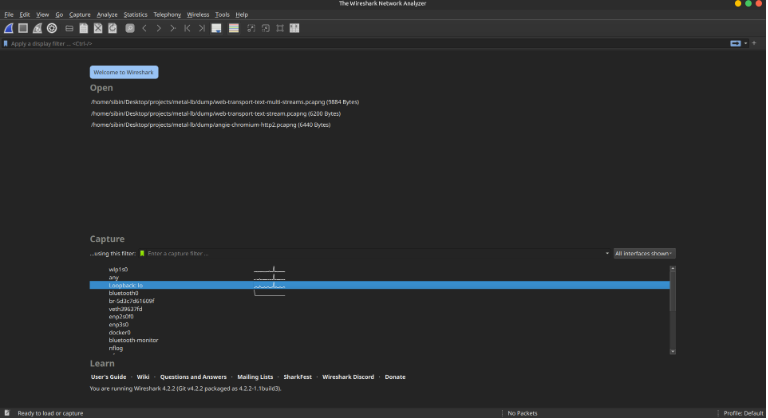
\includegraphics[width=\textwidth]{SOA/ws_interfaces.png}
  \caption{WebSocket Interfaces}
  % \label{fig:ws_interfaces} % optional label for referencing
\end{minipage}
\hfill
\begin{minipage}{0.9\textwidth}
  \centering
  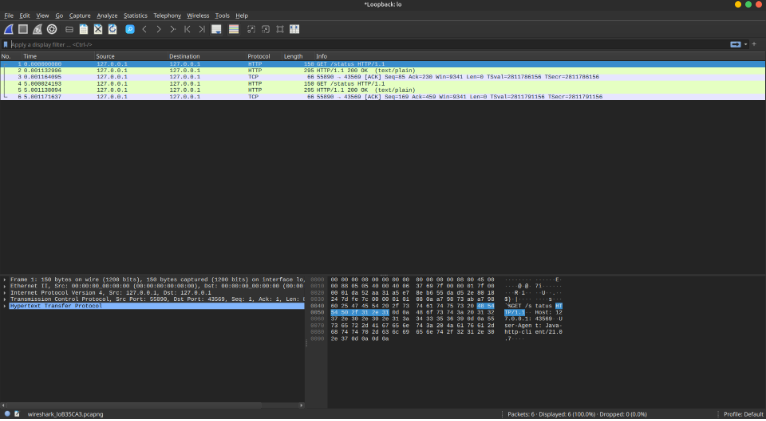
\includegraphics[width=\textwidth]{SOA/ws_packet.png}
  \caption{WebSocket Packets}
  % \label{fig:ws_packet} % optional label for referencing
\end{minipage}
\end{figure}



\section{Containers}
Containers are lightweight, portable, and consistent runtime environments that package an application along with all its dependencies, configuration files, and system libraries. Unlike traditional virtual machines, containers share the host operating system kernel, making them faster to start and more resource-efficient. Containers are created with a container image and all the information is bundled into an image and stored in a registry. This makes it ideal for deploying and scaling applications in a microservices architecture. In context for this dissertation, in order to deploy and run applications in Kubernetes, the prerequisite is having a Docker image ready.

\section{Kubernetes Concepts}
\subsection{Kubernetes Architecture Overview}
Kubernetes is built on a distributed architecture consisting of a Control Plane and multiple Worker Nodes. The Control Plane manages the cluster's desired state and handles decisions such as scheduling, scaling, and responding to cluster events. It includes components like the API Server, etcd (a consistent, distributed key-value store), Scheduler, and Controller Manager. The Control Plane acts as the brain of the system, making high-level decisions and continuously monitoring and adjusting the cluster to match the user-defined configuration.

The Worker Nodes run the actual containerized applications. Each node hosts essential services: the kubelet (which ensures containers are running properly as specified by the control plane), the container runtime (e.g., containerd), and the kube-proxy, which handles networking and service discovery. Kubernetes follows a declarative model, where users define the desired state (like the number of replicas, image versions, etc.), and the system uses control loops to match the actual state with the desired state, ensuring continuous compliance and fault tolerance. Various core components within these layers work together to ensure reliability, scalability, and self-healing of applications across the cluster.

\subsection{Kubernetes Components}
\subsubsection{API Server}
The Kubernetes API Server (kube-apiserver) serves as the central management interface, exposing the Kubernetes API for communication between cluster components and external clients. It processes RESTful requests, validates and stores object configurations (e.g., Pods, Services) in the etcd database, and coordinates cluster operation. Any operation in the cluster goes through the API Server.

\subsubsection{etcd}
etcd is a distributed key-value store that maintains the cluster's configuration and state data, ensuring consistency and fault tolerance. It stores all Kubernetes objects, such as Pod definitions and Service configurations, providing a single source of truth for the control plane. The etcd allows to rollback to a previous cluster state.

\subsubsection{Controller Manager}
The Controller Manager (kube-controller-manager) runs control loops that monitor the cluster's state and match it with the desired state defined in manifests. It includes controllers like the Node Controller (managing node lifecycle), ReplicaSet Controller (ensuring pod replicas), and Service Controller (integrating with load balancers). 

\subsubsection{Scheduler}
The Scheduler (kube-scheduler) assigns pods to nodes based on resource requirements, constraints, and policies (e.g., affinity, taints). It optimizes resource utilization by evaluating node capacity and workload demands. For streaming use cases, the Scheduler ensures that Pulsar brokers or services are placed on nodes with sufficient resources, enhancing performance.

\subsubsection{Kubelet}
The Kubelet, running on each worker node, manages pod lifecycle by communicating with the API Server and container runtime (e.g., containerd, CRI-O). It ensures containers are running, healthy, and configured per pod specifications. In HTTP/3 deployments, Kubelets manage containers hosting QUIC-based services, as seen in prior Angie configurations.

\subsubsection{Kube-Proxy}
Kube-Proxy, also running on worker nodes, manages network rules to enable communication between pods, services, and external clients. It supports modes like iptables and IPVS, facilitating load balancing for services. In this dissertation, MetalLB setup \cite{metallb-docs}, Kube-Proxy worked alongside MetalLB to expose HTTP/3 services via UDP passthrough.

\subsubsection{Container Runtime}
The container runtime (e.g., containerd, CRI-O) executes containers within pods, handling image pulling, container creation, and lifecycle management. It interfaces with the Kubelet to ensure containers adhere to pod specifications.

\subsubsection{Storage Provisioner}
The Storage Provisioner dynamically allocates persistent storage to pods via PersistentVolumeClaims (PVCs) and PersistentVolumes (PVs) (see section 2.6.2.16). It interfaces with storage backends (ie volumes) to provision volumes based on StorageClass definitions. In this dissertation, for Apache Pulsar \cite{pulsar-helm-repo}, the Storage Provisioner ensures bookies have access to persistent storage for ledgers, supporting fault-tolerant data retention. Also configurations, involving MetalLB and Pulsar, relied on Storage Provisioners to manage storage for stateful workloads.

\subsubsection{CoreDNS}
CoreDNS, the default DNS service in Kubernetes, provides service discovery and name resolution within the cluster. Running as a pod, it resolves service names (e.g., http3-service.default.svc.cluster.local) to Pod IP addresses, enabling communication between pods and services. In HTTP/3 deployments, CoreDNS resolves backend service names for QUIC-based traffic, as seen in prior Angie and MetalLB setups. Its plugin-based architecture supports customization, such as integrating with external DNS providers.

\subsubsection{Namespaces}
Namespaces are logical separation of resources into groups. For example, all of the core architecture components run in a separate namespace kube-system.

\subsubsection{Pods}
A Pod is the smallest and simplest unit in the Kubernetes object model. It represents a single instance of a running process in a cluster. A pod can contain one or more containers that share the same network namespace, IP address, and storage volumes. Containers in the same pod can communicate using localhost and share mounted storage, making them ideal for tightly coupled workloads (e.g., a main app container and a sidecar for logging). Pods are ephemeral—once deleted or crashed, they aren't recreated unless managed by a higher-level controller like a Deployment or StatefulSet.


\begin{figure}[H]
\caption{Pods}
\centering
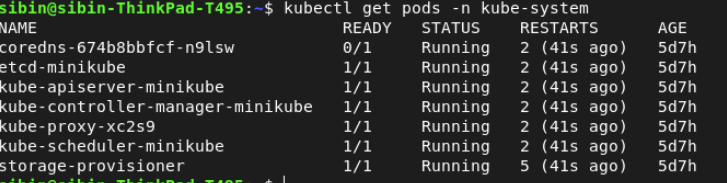
\includegraphics[width=1\textwidth]{SOA/k8s-components.png}
\end{figure}

The above figure shows the pods present in the namespace kube-system

\subsubsection{Deployments}
A Deployment is a controller that manages the lifecycle of pods. It ensures the desired number of pod replicas are running and updates them in a controlled manner. With deployments, users can perform rolling updates, rollbacks, and maintain zero downtime during application changes. When you update a deployment (e.g., to use a new container image), Kubernetes gradually replaces the old pods with new ones, ensuring stability throughout the process. Deployments abstract the complexity of pod creation and replication, offering scalability and resilience.

\begin{figure}[H]
\caption{Deployments}
\centering
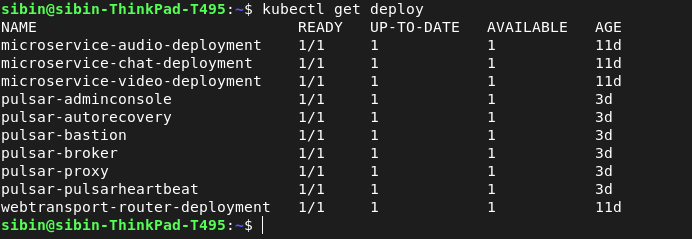
\includegraphics[width=1\textwidth]{SOA/k_deploy.png}
\end{figure}
The above figure illustrates the different deployment in the cluster's default namespace

\subsubsection{Services}
Kubernetes Services provide a stable networking endpoint to access pods, abstracting away their transient nature. Since pods have dynamic IPs and may be replaced, services ensure that applications or users can access workloads reliably. There are several types of services:

\begin{itemize}
    \item ClusterIP (default): Exposes the service on a cluster-internal IP. It is only accessible within the cluster, useful for internal communication between services.
    \item NodePort: Exposes the service on a static port (between 30000–32767) on each worker node's IP. Traffic to this port is forwarded to the underlying pods. It makes services accessible outside the cluster using  NodeIP:NodePort.
    \item LoadBalancer: Provisions an external load balancer (in cloud environments like Amazon Web Services (AWS) or Google Cloud Platform (GCP)) and routes traffic from the external world to the service. It provides a single external IP and balances traffic to the appropriate pods.
\end{itemize}

\begin{figure}[H]
\caption{Service}
\centering
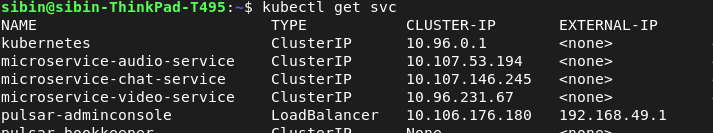
\includegraphics[width=1\textwidth]{SOA/k_svc.png}
\end{figure}
The above figure shows the services present in our cluster in default namespace.


If we are working with an internal service, go for default ClusterIP, and if you want to expose the service to the outside world, use NodePort or LoadBalancer.

\subsubsection{ConfigMaps}
ConfigMaps allows to externalize configuration from container images, separating application code from configuration data. They store key-value pairs that can be used to inject environment variables, command-line arguments, or configuration files into pods. This decoupling allows the same container image to be reused in different environments by simply changing the ConfigMap. For example, you could store database URLs, feature flags, or app settings without baking them into the container. In implementation microservice container image was deployed with config map.

\subsubsection{Secrets}
Secrets are similar to ConfigMaps but designed specifically for sensitive data like passwords, tokens, SSH keys, or certificates. Secrets are base64-encoded (not encrypted by default) and can be mounted as volumes or exposed as environment variables. They help protect confidential data by controlling access through RBAC and reducing the risk of hardcoding secrets into application images or code.

\subsubsection{Persistent Volumes (PVs) and Persistent Volume Claims (PVCs)}
Kubernetes provides an abstraction layer for storage through Persistent Volumes (PVs) and Persistent Volume Claims (PVCs). A PV is a piece of storage (e.g., a disk in a cloud provider or an NFS mount) provisioned by an admin or dynamically via StorageClasses. A PVC is a user's request for storage with specific requirements (like size, access mode).

This decouples storage provisioning from storage consumption, allowing pods to request storage without knowing the details of the underlying storage infrastructure. PVs can outlive pods and enable stateful applications like databases to persist data even when pods are recreated.

\subsubsection{StatefulSets}
StatefulSets are a Kubernetes controller used to manage stateful applications that require stable network identities and persistent storage. Unlike Deployments, which treat all pods as interchangeable, StatefulSets assign each pod a unique, stable identity (including name and network address) and ensure ordered, graceful deployment, scaling, and deletion.

StatefulSets are ideal for workloads like databases (e.g., MongoDB, PostgreSQL), distributed systems (e.g., Kafka, ZooKeeper \cite{zookeeper-docs}), and any application that requires persistent storage tied to a specific pod. Each pod in a StatefulSet can be connected via a predictable DNS name and retains its associated PVC even when restarted.

\subsection{Cloud Kubernetes Clusters}
As Kubernetes adoption continues to rise across industries, cloud providers have responded with fully managed solutions to simplify deployment, scaling, and maintenance. Among the most prominent managed Kubernetes offerings are Amazon Elastic Kubernetes Service (EKS), Azure Kubernetes Service (AKS), and Google Kubernetes Engine (GKE). This section reviews these platforms, examining their design principles, cloud integration capabilities, and recent developments, with a focus on their maturity and positioning in the cloud-native ecosystem.

\subsubsection{EKS}
Amazon Elastic Kubernetes Service (EKS), introduced by AWS in 2018, offers a fully managed control plane that spans multiple Availability Zones to ensure high availability and resilience \cite{aws-docs}. It leverages the security and scalability of AWS infrastructure while supporting native Kubernetes tooling. EKS integrates tightly with AWS services such as Identity and Access Management (IAM) for access control, CloudWatch for observability, and Elastic Load Balancer (ELB) for load balancing. Recent additions like EKS Anywhere (for on-premises Kubernetes) and Bottlerocket (a container-optimized OS) reflect AWS's commitment to extending Kubernetes beyond cloud boundaries (AWS, 2025). However, EKS has historically been more complex to configure than its competitors, particularly due to its networking model, which tightly couples pods to Virtual Private Cloud (VPC) configurations (Smith & Alqahtani, 2024).

\subsubsection{AKS}
Azure Kubernetes Service (AKS) represents Microsoft's managed Kubernetes platform and is particularly favored in enterprise environments with existing Azure investments \cite{azure-docs}. AKS manages the Kubernetes control plane free of cost and supports features like node auto-scaling, Azure Active Directory (AD) integration, and Virtual Node support via Azure Container Instances (ACI). As of 2025, Microsoft has enhanced its hybrid cloud capabilities through Azure Arc, enabling consistent Kubernetes management across cloud and on-prem infrastructure (Microsoft Docs, 2025). Though AKS is generally user-friendly and well-integrated with Azure DevOps and Visual Studio, it sometimes lags behind Google Kubernetes Engine (GKE) in offering the latest Kubernetes versions (Nguyen et al., 2023).

\subsubsection{GKE}
GKE is widely considered the most advanced managed Kubernetes platform, owing to Google's foundational role in developing Kubernetes \cite{gcp-docs}. It offers both a Standard mode (with user-managed nodes) and Autopilot mode, where Google handles infrastructure completely. GKE is known for its rapid adoption of upstream Kubernetes versions, robust autoscaling features (including vertical and horizontal autoscaling), and seamless integration with Istio, Anthos, and Cloud Monitoring. In 2025, GKE continues to be the platform of choice for use cases involving AI/ML and latency-sensitive applications, driven by GCP's high-performance network and container runtime optimizations. However, the opinionated nature of GKE Autopilot may limit low-level customization, which could be a drawback for advanced users.

\subsection{Comparison of Cloud Clusters}
\begin{table}[h]
\small
\centering
\begin{tabular}{|p{3cm}|p{3.5cm}|p{3.5cm}|p{3.5cm}|}
\hline
\textbf{Aspect} & \textbf{Amazon EKS} & \textbf{Azure AKS} & \textbf{Google GKE} \\
\hline
Learning Curve & Steep & Easy for Azure users & Very user-friendly \\
Flexibility & High & Moderate & Lower in Autopilot mode \\
Hybrid Cloud & EKS Anywhere & Azure Arc & Anthos \\
K8s Feature Updates & Slower & Slight delay & Fastest \\
Control Plane Cost (EU/hour) & \$0.10 & Free & \$0.10 (Standard), Free (Autopilot) \\
Minimum Monthly Cost (1 node) & \textasciitilde\$37 (t3.small + control plane) & \textasciitilde\$27 (B2s, free control plane) & \textasciitilde\$30 (e2-small, Autopilot includes control plane) \\
\hline
\end{tabular}
\caption{Simplified Comparison of Kubernetes Cloud Services with Cost Estimates (EU Region)}
\end{table}




More or less, all Kubernetes services offer similar core functions because they all use the open-source Kubernetes implementation. The main differences come from how well they fit specific use cases and how easily they integrate with other tools and services you use. Another big factor when choosing a service is the cost.

Running Kubernetes on managed cloud platforms like EKS, AKS, and GKE can quickly become expensive. Costs include not only the control plane and worker nodes but also storage, networking, and extra monitoring or logging services. Even running a small cluster can cost several hundred dollars a month, which is often too high for students, researchers, or small projects with limited budgets. These expenses make it difficult to experiment freely or run many tests without worrying about costs. Because of this, managed cloud Kubernetes may not always be the best choice for those just learning or developing smaller projects.

Instead, leaning towards a local Kubernetes solution would be much more beneficial. It allows users to experiment, learn, and develop without the pressure of high cloud costs. This approach makes it easier to try different configurations and troubleshoot problems without incurring unexpected expenses. For educational or early-stage projects, this flexibility can be a significant advantage.

\subsection{Local Kubernetes Cluster}
Due to the high cost of managed Kubernetes services, especially for smaller research or academic projects, local Kubernetes setups have become the preferred and practical alternative. Running clusters locally avoids the ongoing expenses of cloud infrastructure and gives developers full control over their environments. While exposing services or configuring networking can take more effort, local clusters help in understanding the inner workings of Kubernetes, making them valuable for hands-on learning and experimentation. Today, local clusters are widely used in educational, testing, and CI/CD environments, making them a state-of-the-art solution for development purposes. This section explores three widely adopted tools used for local Kubernetes deployments: Minikube, kind, and K3s.

\subsubsection{Minikube}
Minikube is one of the most widely used tools for spinning up a local Kubernetes cluster \cite{minikube-docs}. It supports running a single-node cluster inside a VM or container and works on Windows, macOS, and Linux. Minikube offers a rich set of built-in features like a Kubernetes dashboard, Ingress controllers, metrics-server, and support for multiple drivers (VirtualBox, Docker, etc.). It also allows testing across different Kubernetes versions. The documentation is well maintained, and the active user community makes troubleshooting and learning much easier. These characteristics make Minikube a solid choice for learners, developers, and small project environments.

\subsubsection{kind}
Kind (Kubernetes IN Docker) is a fast and lightweight tool that runs Kubernetes clusters inside Docker containers \cite{kind-docs}. It's designed mainly for testing Kubernetes itself or running automated CI/CD pipelines. Kind is quick to start and destroy, making it ideal for scenarios where clusters need to be recreated often. However, it doesn't provide many built-in add-ons, and setting up networking features like Ingress or LoadBalancer typically needs more manual configuration. Kind is more suitable for automated testing than hands-on experimentation with services or full-featured deployments.

\subsubsection{K3s}
K3s is a lightweight Kubernetes distribution developed by Rancher and optimized for low-resource environments such as edge devices and IoT systems \cite{k3s-docs}. Despite being compact, K3s remains fully Kubernetes-compliant and supports modern features like Helm charts and CRDs. It is often used in production for small clusters, thanks to its low memory usage and simplified installation. While K3s is powerful, it may not be the best starting point for new users due to its minimal abstraction and less emphasis on beginner documentation.

\subsection{Local Clusters Comparison}
\begin{table}[h]
\centering
\begin{tabular}{|l|c|c|c|}
\hline
\textbf{Aspect} & \textbf{Minikube} & \textbf{kind} & \textbf{K3s} \\
\hline
Setup & Easy & Very Easy & Moderate \\
Use Case & Learning / Dev & CI/CD Testing & Edge / IoT \\
Add-ons & Built-in & Manual setup & Limited \\
Performance & Moderate & Fast & Very Lightweight \\
Community & Large & Niche & Growing \\
\hline
\end{tabular}
\caption{Simplified Comparison of Local Kubernetes Clusters}
\end{table}


After comparing all three tools, it was decided to proceed with Minikube for this project. It offers the best balance between usability, features, and support. The wide range of add-ons made it easier to test application deployments, networking policies, and configuration setups. Its clear documentation and active support community also reduces the time spent on troubleshooting. Although kind and K3s are also capable tools, Minikube gave us the flexibility needed to experiment freely in a cost-effective and controlled environment.

ALl of the internal component communication in the local clusters are based in TCP and HTTP 1.1. Neither of the Kubernetes solutions support forwarding QUIC connections natively hence, alternative workarounds are needed.

\subsection{Custom Resource Definitions (CRDs)}
Custom Resource Definitions (CRDs) let users add new types of objects to Kubernetes, such as Gateway API (see section 2.6.10). These custom resources behave like built-in ones (e.g., Pods, Services), allowing teams to manage them using tools like kubectl. A CRD only defines the structure of a custom resource. To make it work, a separate program called a controller watches for changes and performs actions to match the desired state. Controllers are often built using tools like Kubebuilder or Operator SDK.

CRDs are widely used in tools like Prometheus Operator to automate tasks and manage infrastructure. While building controllers can be complex, they allow teams to create powerful, reusable, and automated workflows inside Kubernetes. In this project, CRDs help manage Apache Pulsar clusters automatically within Kubernetes, making deployment and scaling much easier.

\subsection{Ingress Controllers in Kubernetes}
An Ingress Controller is a critical component in Kubernetes used to expose services, APIs, or web applications running inside the cluster to external users over HTTP or HTTPS. It works alongside Ingress resources, which define routing rules, to manage how external requests reach internal services. While Kubernetes provides the Ingress resource as part of its API, it does not ship with a default controller—users must install and configure one manually. Ingress controllers interpret these rules and handle tasks such as URL-based routing, TLS termination, and load balancing, enabling scalable, declarative web and API access. The different types of ingress controllers are as follows:



For platform-independent or more advanced use cases, several third-party ingress controllers are widely adopted. The NGINX Ingress Controller is the most common, known for its flexibility and ease of use across any Kubernetes setup. Traefik is a modern alternative that auto-discovers services and integrates well into dynamic or CI/CD-heavy environments. For API-first architectures, the Kong Ingress Controller doubles as an API gateway, offering authentication, rate limiting, and monitoring features. Istio's Ingress Gateway, designed for service meshes, provides advanced capabilities like mTLS, circuit breaking, and traffic splitting—ideal for secure, production-grade microservices deployments.

The following is the syntax for ingress controllers
\begin{lstlisting}[language=yaml]
apiVersion: networking.k8s.io/v1
kind: Ingress
metadata:
  name: example-ingress
  annotations:                        # (Controller-specific customizations go here)
    <controller-specific-annotations>
spec:
  ingressClassName: <controller-name>  # (Name of the ingress class, like nginx, alb, kong)
  rules:
  - host: <your-domain.com>
    http:
      paths:
      - path: /                       # (URL path prefix to match)
        pathType: Prefix              # (Usually Prefix or Exact)
        backend:
          service:
            name: <service-name>     # (Your Kubernetes service name)
            port:
              number: <port-number>  # (Service port to route traffic to)
\end{lstlisting}
Here we would use the custom annotations for the specific ingress we will use.


\subsection{Ingress Controller Support for HTTP/3 and QUIC}
HTTP/3, the latest evolution of the HTTP protocol, brings significant advantages in performance and reliability by using QUIC, a transport protocol that operates over UDP and integrates TLS 1.3. Despite growing interest in HTTP/3 for its benefits—such as reduced latency and improved multiplexing—Kubernetes Ingress Controllers have been slow to adopt it due to technical challenges and architectural limitations.

Most widely-used Ingress Controllers, like NGINX and HAProxy, are based on traditional HTTP/1.1 and HTTP/2 over TCP. Since HTTP/3 relies on QUIC, it requires support for UDP, TLS 1.3, and specialized libraries like BoringSSL. These changes involve substantial rewrites of existing proxying logic and networking layers, making native support difficult. As a result, HTTP/3 functionality in Kubernetes Ingress Controllers is generally experimental, requiring custom builds, complex configuration, and lack of standardization across implementations.


\subsubsection{NGINX Ingress Controller and HTTP/3 Support}

NGINX Ingress Controller is one of the most widely adopted ingress controllers in Kubernetes \cite{nginx-ingress-docs}. However, its official support for HTTP/3 remains limited and somewhat unclear. The official NGINX Ingress Controller documentation lacks a straightforward guide for enabling HTTP/3, making configuration challenging for users attempting to adopt this protocol.

At the core, HTTP/3 support in the underlying NGINX web server is provided via the \texttt{ngx\_http\_v3\_module}, which has been available since NGINX version 1.25.0. However, this module is \textbf{not built into the official NGINX package by default}. Enabling HTTP/3 requires compiling NGINX from source with the \texttt{--with-http\_v3\_module} flag and linking it against a QUIC-compatible TLS library such as \textbf{BoringSSL} or \textbf{QuicTLS}. This setup is more feasible at the web server level than within the Kubernetes-managed ingress controller.

To investigate support at the Kubernetes ingress level, attempts were made to pass relevant parameters via Helm during deployment:

\begin{verbatim}
helm install ingress-nginx ingress-nginx/ingress-nginx \
  --namespace ingress-nginx --create-namespace
\end{verbatim}

This opened TCP ports in the service. To enable QUIC support, UDP traffic must also be allowed to reach the ingress. Therefore, the following patch was applied to the service to expose UDP on port 443:

\begin{verbatim}
kubectl patch svc ingress-nginx-controller -n ingress-nginx \
  --type='json' -p='[{"op": "add", "path": "/spec/ports/-", 
  "value": {"name":"quic","port":443,"protocol":"UDP","targetPort":443}}]'
\end{verbatim}

In the latest versions of the NGINX Ingress Controller, the HTTP/3 module appears to be compiled in by default. Additional configurations to expose QUIC via UDP were attempted.

Despite these configurations, the ingress controller does not currently provide sufficient mechanisms to fully inject QUIC and HTTP/3 configuration parameters within a Kubernetes environment, as the NGINX Ingress Controller does not support any specific flags for QUIC behavior. There are \textbf{no officially supported parameters} to manage QUIC-specific settings or negotiate HTTP/3 connections reliably. As a result, while partial support exists at the NGINX core level, the NGINX Ingress Controller's HTTP/3 capabilities remain \textbf{experimental and limited} in practical Kubernetes deployments.



\subsubsection{HAProxy Ingress Controller and HTTP3 Support}
HAProxy has introduced experimental HTTP/3 support starting with version 2.6 \cite{haproxy-docs} \cite{haproxy-k8s-docs}. Its Ingress Controller can leverage this functionality. This includes enabling UDP listeners, tuning TLS settings, and adjusting protocol stacks manually—none of which are typically available through standard Helm charts. 


To test HTTP/3 support in a Kubernetes environment, the following steps were performed:

\begin{enumerate}
  \item The HAProxy Helm repository was added and updated:
  \begin{verbatim}
  helm repo add haproxytech https://haproxytech.github.io/helm-charts
  helm repo update
  \end{verbatim}

  \item The HAProxy ingress controller was installed with a custom values file:
  \begin{verbatim}
  helm install haproxy-quic haproxytech/kubernetes-ingress -f haproxy-quic-values.yaml
  \end{verbatim}

  In the \texttt{haproxy-quic-values.yaml} file, the configuration exposed UDP port 443 and passed the flag \texttt{--quic-bind-port=443} to enable QUIC and HTTP/3 support.

  \item An \texttt{Ingress} resource was applied, using the HAProxy ingress class and pointing to a backend service. A self-signed TLS certificate was used with the hostname \texttt{quic-aioquic.com}.
\end{enumerate}

Once deployed, HTTP/3 functionality was tested using \texttt{curl}:

\begin{verbatim}
curl --http3-only --verbose --insecure https://192.168.49.4 \
  -H "Host: quic-aioquic.com"
\end{verbatim}

The response confirmed that HTTP/3 was successfully negotiated. However, backend service logs indicated that the request was received using HTTP/1.1:

\begin{verbatim}
10.244.1.122 - - [07/Aug/2025:12:55:39 +0000] "GET / HTTP/1.1" ...
\end{verbatim}

This confirms that HAProxy terminates the HTTP/3 connection and opens a new one to the backend using a lower protocol version.

\paragraph{Limitations.}
Although HAProxy can accept HTTP/3 connections from clients, it does not forward them using HTTP/3 to backend services. The ingress controller does not support inspecting or demultiplexing QUIC packets. As a result, HTTP/3 is only supported at the edge, and end-to-end HTTP/3 communication within Kubernetes is not yet feasible using HAProxy.



\subsubsection{Workarounds}
Given the lack of mature, native HTTP/3 support in mainstream Ingress Controllers, it is currently more practical to experiment with HTTP/3 directly at the web server level for Nginx and Traefic which wasnt able to support ingress like ha-proxy. We will look at the webserber Angie which is a fork of nginx especially created for h3 support in section

\subsection{Gateway API}
\subsubsection{Overview}
The Gateway API is a recent advancement in Kubernetes networking designed to address the limitations of the traditional Ingress API. While Ingress has served as the de facto method for managing external traffic into Kubernetes clusters, it suffers from inflexibility, heavy reliance on annotations, and poor support for non-HTTP protocols. The Gateway API introduces a more robust, extensible, and protocol-agnostic model that allows infrastructure operators and application developers to define their concerns independently, thus supporting multi-tenancy and complex networking scenarios more effectively.

One of the defining features of the Gateway API is its emphasis on supporting a wide variety of protocols beyond HTTP and HTTPS, such as TCP and UDP, with emerging support for QUIC and HTTP/3. This makes the API particularly relevant for modern, low-latency, and multiplexed applications that demand richer transport capabilities. The architecture facilitates this through a set of Kubernetes-native Custom Resource Definitions (CRDs), allowing developers and operators to interact with networking policies declaratively and with clear separation of responsibilities.


\subsubsection{Architecture and Core Components}
The Gateway API introduces modular CRDs for fine-grained network traffic control in Kubernetes. GatewayClass defines types of gateways (e.g., Envoy, HAProxy), managed by admins, while Gateway instances configure ports, protocols, and TLS settings. Routing is handled by resources like HTTPRoute, TCPRoute, and UDPRoute, which forward traffic based on specific rules. Additional resources like ReferencePolicy support cross-namespace and security configurations. This design separates infrastructure and application concerns, improving scalability, security, and maintainability


\subsubsection{Gateway API Implementation for HTTP3 Support}

Since HAProxy successfully worked with Ingress for HTTP/3 forwarding, the next step was to implement the Gateway API using the HAProxy controller.

\subsubsubsection{Installing the HAProxy Gateway Controller}

The following steps were performed:

\begin{itemize}
  \item Added the Helm repository:
\begin{lstlisting}[language=bash]
helm repo add haproxytech https://haproxytech.github.io/helm-charts
helm repo update
\end{lstlisting}

  \item Installed the controller with Gateway API support:
\begin{lstlisting}[language=bash]
helm install haproxy-gateway-controller haproxytech/kubernetes-ingress \
  --namespace haproxy-gateway-system --create-namespace \
  --set controller.kubernetesGateway.enabled=true \
  --set controller.kubernetesGateway.gatewayControllerName=haproxy.org/gateway-controller \
  --set controller.service.type=LoadBalancer
\end{lstlisting}
\end{itemize}

Once deployed, a LoadBalancer service was exposed, including a UDP port for QUIC:

\begin{lstlisting}[language=bash]
NAME                                            TYPE           CLUSTER-IP     EXTERNAL-IP    PORT(S)                                                                  AGE
haproxy-gateway-controller-kubernetes-ingress   LoadBalancer   10.104.20.31   192.168.49.5   80:31433/TCP,443:32261/TCP,443:32261/UDP,1024:30450/TCP,6060:31286/TCP   117s
\end{lstlisting}

\subsubsection{Defining the Gateway}

The Gateway resource was created to expose HTTPS and QUIC traffic:

\begin{lstlisting}[language=yaml]
apiVersion: gateway.networking.k8s.io/v1
kind: Gateway
metadata:
  name: haproxy-gateway
spec:
  gatewayClassName: haproxy
  listeners:
  - name: https
    protocol: HTTPS
    port: 443
    tls:
      mode: Terminate
      certificateRefs:
      - kind: Secret
        name: your-tls-secret
  - name: quic
    protocol: HTTPS
    port: 443
    tls:
      mode: Terminate
      certificateRefs:
      - kind: Secret
        name: your-tls-secret
\end{lstlisting}

\subsubsection{Defining the HTTPRoute}

An HTTPRoute was defined to route requests based on hostname:

\begin{lstlisting}[language=yaml]
apiVersion: gateway.networking.k8s.io/v1
kind: HTTPRoute
metadata:
  name: haproxy-http3-route
spec:
  parentRefs:
  - name: haproxy-gateway
    sectionName: https-quic
  hostnames:
  - "gateway-haproxy.com"
  rules:
  - backendRefs:
    - name: http3-test
      port: 80
\end{lstlisting}

\subsubsection{Packet Flow Description}

The observed packet flow is as follows:

\begin{itemize}
  \item Client sends request to LoadBalancer service.
  \item The HAProxy pod receives the request, decrypts it using the TLS certificate.
  \item It matches the hostname and routes the request based on the Gateway and Route configuration.
  \item The request is forwarded to the backend service.
\end{itemize}

\subsubsection{Operational Separation}

The Gateway API introduces a clean separation of responsibilities:
\begin{itemize}
  \item \textbf{Infrastructure providers} manage the GatewayClass resources (e.g., HAProxy, NGINX).
  \item \textbf{Cluster administrators} handle gateway resources (TLS, listeners, ports).
  \item \textbf{Application developers} define HTTPRoute or TCPRoute objects, configuring hostnames and routing rules.
\end{itemize}

This separation encourages better scalability and maintainability in Kubernetes environments.

\subsubsection{Observed Limitation in HTTP/3 Stream Handling}

While the Gateway API supports HTTP/3 and correctly forwards such requests to backend services, a limitation was observed:

When HTTP/3 requests are made, the Gateway forwards them correctly, showing basic QUIC support. However, similar to the behavior of the HAProxy Ingress Controller, the Gateway API treats the request as a single unit. There is no visibility or control over individual HTTP/3 streams.

This indicates that the Gateway API currently lacks support for stream-level features of HTTP/3. It does not provide insight into or allow manipulation of separate streams within a connection. Therefore, the full capabilities of HTTP/3, such as fine-grained stream-level routing or observation, are not realized.

\subsubsection{Declarative Configuration vs. Annotation-Driven Models}
A major improvement introduced by the Gateway API is its declarative configuration model, which replaces the annotation-heavy approach of the traditional Ingress API. Annotations in Ingress controllers often lack standardization, are implementation-specific, and are difficult to validate, leading to operational ambiguity. In contrast, the Gateway API uses structured CRDs to define listeners, routes, and policies, making configuration clearer, more consistent, and easier to validate.

Nevertheless, annotations have not been entirely eliminated. They are still used in specific cases, particularly to enable experimental features or for backward compatibility with legacy tooling. For example, enabling QUIC support or selecting specific cipher suites via BoringSSL may still require annotations, depending on the controller. However, these annotations are supplementary rather than central, with the primary configuration expressed through first-class Kubernetes resources. This allows for richer multi-protocol configurations—such as defining a single gateway that supports both TCPRoute and UDPRoute—an arrangement difficult to express using traditional Ingress.


\subsection{QUIC Library Implementations: Aioquic, Quic-go, and Quiche}
The standardization of the QUIC protocol by the IETF has encouraged the development of several independent and open-source implementations to support integration across diverse ecosystems. These implementations serve not only as vehicles for QUIC protocol adoption but also as platforms for experimentation, optimization, and integration into real-world systems. Among the most prominent and actively maintained QUIC libraries are Aioquic, Quic-go, and Quiche, each developed in a distinct programming language and suited to particular performance and deployment goals. This section provides a detailed examination of these libraries, discussing their internal architecture, design philosophies, and practical usage in production or research environments.

\subsubsection{Aioquic}
Aioquic is a Python-based implementation of the QUIC and HTTP/3 protocols developed by aiortc, and is designed to provide asynchronous, non-blocking I/O through Python's asyncio framework. Aioquic is particularly well-suited to academic and research applications due to its readability, high-level abstractions, and ease of integration within Python-based systems. It supports essential QUIC features such as stream multiplexing, TLS 1.3 handshake, connection migration, datagram frames, 0-RTT resumption, and HTTP/3 protocol negotiation.

\paragraph{Architecture and Design}
At the core of Aioquic lies an event-driven state machine that responds to received packets and timer expirations. It integrates closely with Python's asyncio event loop, allowing developers to implement clients and servers that handle concurrent connections efficiently using coroutines. The QuicConnection class encapsulates the transport logic, while the H3Connection class manages the HTTP/3 layer on top of QUIC streams. Developers can subclass the QuicConnectionProtocol to customize behavior for server-side or client-side implementations.

Aioquic also includes built-in support for logging using qlog, a standardized QUIC tracing format. This enhances its suitability for debugging and protocol analysis. In terms of modularity, the library is structured to allow developers to use just the QUIC transport layer or to integrate HTTP/3 as needed, making it flexible for building custom protocols atop QUIC.

\paragraph{Implementation Example}
A typical Aioquic application involves initializing a QUIC configuration, creating a connection context, and using asynchronous tasks to send and receive data. Below is a simplified example of a client establishing a secure QUIC connection and sending data over a stream:

\begin{lstlisting}[language=python]
from aioquic.asyncio import connect
from aioquic.quic.configuration import QuicConfiguration
import asyncio

async def main():
    configuration = QuicConfiguration(is_client=True)
    async with connect("example.com", 4433, configuration=configuration) as protocol:
        stream_id = protocol._quic.get_next_available_stream_id()
        protocol._quic.send_stream_data(stream_id, b"Hello, QUIC!", end_stream=True)
        await protocol.wait_closed()

asyncio.run(main())
\end{lstlisting}

This minimal example illustrates Aioquic's ease of use and is indicative of how rapidly developers can prototype with the library.

\paragraph{Use Cases and Adoption}
While Aioquic is not yet widely deployed in commercial production environments due to Python's performance limitations, it is frequently used in academic research, protocol testing, and rapid prototyping.

\subsubsection{Quic-go}
Quic-go is a Go-based implementation of the QUIC protocol, maintained by the open-source community and initially developed by lucas-clemente, with substantial contributions from the Chromium networking team. Quic-go is designed for robustness and performance and has been widely integrated into real-world systems, including browsers and cloud-native applications.

\paragraph{Architecture and Design}
Quic-go leverages Go's lightweight concurrency model through goroutines and channels, making it highly scalable for managing thousands of concurrent QUIC sessions. The library adheres closely to the IETF QUIC specification and includes a complete implementation of HTTP/3, along with transport features such as packet pacing, congestion control (CUBIC, BBR), retransmissions, connection ID rotation, stateless resets, and forward error correction (FEC).

The internal architecture comprises multiple interacting subsystems: the connection package manages connection-level state, streams handles stream multiplexing, and ackhandler is responsible for packet acknowledgment and retransmission tracking. The integration of Go's cryptographic primitives allows native handling of TLS 1.3 through the crypto/tls library.

\paragraph{Implementation Example}
The following snippet illustrates a basic QUIC server using Quic-go, which listens for incoming connections and echoes received data:

\begin{lstlisting}[language=go]
package main

import (
    "crypto/tls"
    "github.com/quic-go/quic-go"
    "io"
    "log"
)

func main() {
    tlsConf := &tls.Config{
        Certificates: []tls.Certificate{loadTLSCertificate()},
        NextProtos:   []string{"h3"},
    }

    listener, err := quic.ListenAddr(":4242", tlsConf, nil)
    if err != nil {
        log.Fatal(err)
    }

    for {
        sess, err := listener.Accept(nil)
        if err != nil {
            log.Fatal(err)
        }
        go handleSession(sess)
    }
}

func handleSession(sess quic.Connection) {
    stream, err := sess.AcceptStream(nil)
    if err != nil {
        log.Println(err)
        return
    }
    io.Copy(stream, stream) // Echo
}
\end{lstlisting}

This example demonstrates how Quic-go abstracts away low-level networking concerns, allowing developers to focus on application logic.

\paragraph{Use Cases and Adoption}
Quic-go is embedded in the Chromium browser stack, where it underpins HTTP/3 communication. It has also been adopted in several high-throughput applications, including Caddy, a modern Go-based web server, and FrankenQUIC, a QUIC protocol experimentation platform. Its production-readiness and active maintenance make it an excellent choice for developers building scalable, network-intensive applications in the Go ecosystem.

\subsubsection{Quiche}
Quiche is a QUIC and HTTP/3 implementation written in Rust by Cloudflare, focusing on performance, security, and integration into high-speed, production-grade systems. Quiche is used extensively within Cloudflare's global CDN infrastructure, where it handles millions of QUIC connections across edge locations.

\paragraph{Architecture and Design}
Quiche benefits from Rust's safety guarantees and zero-cost abstractions, which make it ideal for low-level network programming. The library is designed to operate as a "no-std" Rust crate, enabling usage in environments with limited standard library support (e.g., embedded systems or unikernels).

The architecture revolves around a stateful Connection object, which manages packet parsing, stream states, congestion control, and cryptographic negotiation. The library implements advanced features such as 0-RTT data resumption, QPACK header compression, packet coalescing, and stream prioritization. Quiche also offers tight integration with qlog tracing and supports ALPN negotiation for HTTP/3 and custom application protocols.

Quiche is built to be embedded into other C/C++/Rust programs via its Foreign Function Interface (FFI), making it highly versatile.

\paragraph{Implementation Example}
A basic HTTP/3 server using Quiche is more complex due to Rust's strict safety model, but the following pseudocode outlines the core flow:

\begin{lstlisting}[language=rust]
let mut conn = quiche::accept(&scid, None, local_addr, peer_addr, &mut config)?;
let (read, _) = socket.recv_from(&mut buf)?;
let recv_info = quiche::RecvInfo { from: peer_addr, to: local_addr };

conn.recv(&mut buf[..read], recv_info)?;

if conn.is_established() {
    if let Ok((stream_id, data)) = conn.readable().next() {
        // Process stream data
    }
}
\end{lstlisting}

This example shows the control developers have over connection handling and packet flow when using Quiche.

\paragraph{Use Cases and Adoption}
Quiche is used in Cloudflare's HTTP/3 infrastructure and has been integrated into major projects such as Nginx, curl, and Wireshark (for traffic analysis). Its adoption by performance-critical applications highlights its production maturity and scalability. Additionally, its inclusion in the QUIC Interop Runner and extensive qlog support make it a valuable reference implementation for QUIC protocol conformance testing.

\subsubsection{Summary of Libraries}
The three libraries—Aioquic \cite{aioquic-repo}, Quic-go \cite{quic-go-repo}, and Quiche \cite{quiche-repo} explains the diversity of QUIC implementations, each targeting different domains. Aioquic prioritizes accessibility and research flexibility whereas Quic-go balances performance and developer usability and finally Quiche focuses on high-throughput, secure, production deployments. The choice among them depends on the development environment, performance constraints, and programming language expertise. In the context of this dissertation, Aioquic is selected for the implementation phase because of its easy syntax.  ie. Python being easy to understand and configure.

\subsection{Angie Webserver}
Angie is a high-performance, modular web server and reverse proxy developed as a fork of NGINX, with explicit focus on supporting emerging protocols and modern web traffic patterns \cite{angie-docs}. One of Angie's key differentiators is its support for HTTP/3 via native QUIC integration. By leveraging QUIC, Angie can handle low-latency, multiplexed connections over UDP, making it suitable for next-generation web workloads. Angie's modular architecture also facilitates extensibility for protocol enhancements and security mechanisms.

In this study, Angie was deployed within a Kubernetes environment using the official container image (docker.angie.software/angie:latest). Configuration was managed via a Kubernetes ConfigMap, specifying server blocks, TLS settings, and QUIC-related directives. Angie successfully forwarded HTTP/3 traffic to backend services, validating its compatibility with QUIC at the connection level. However, its current implementation lacks the ability to perform stream-level inspection or manipulation within QUIC connections. This limits its support for finer-grained traffic control and observability across individual HTTP/3 streams which is feature critical for advanced routing, security policies, and telemetry in production environments.

Despite these limitations, Angie presents a stable and efficient reverse proxy solution for HTTP/3 traffic, suitable for experimental deployments and scenarios where basic QUIC forwarding suffices. Its adherence to evolving protocol standards and active development trajectory make it a compelling candidate for future-ready capable proxy.

\subsubsection{Angie Configuration for HTTP/3 Forwarding}
Angie's architecture supports HTTP/3 by enabling QUIC listeners alongside traditional TCP listeners. The proxy was deployed Angie using the Docker image docker.angie.software/angie:latest in a Kubernetes environment, configured via a ConfigMap as shown below:

\begin{lstlisting}[language=yaml]
apiVersion: v1
kind: ConfigMap
metadata:
  name: angie-config
data:
  angie.conf: |
    worker_processes auto;
    events {}
    http {
      log_format detailed '$remote_addr - $remote_user [$time_local] '
                          '"$request" $status $body_bytes_sent '
                          '"$http_referer" "$http_user_agent" '
                          'protocol=$server_protocol http3=$http3';
      access_log /dev/stdout detailed;
      server {
        listen 443 ssl;
        listen 443 quic reuseport;
        ssl_certificate     /certs/tls.crt;
        ssl_certificate_key /certs/tls.key;
        add_header Alt-Svc 'h3=":443"; ma=86400; persist=1';
        ssl_protocols TLSv1.3;
        ssl_ciphers HIGH:!aNULL:!MD5;
        ssl_prefer_server_ciphers on;
        http2 on;
        location / {
          return 200 "Hello from Angie via HTTP/3!\n";
        }
        location /service {
          proxy_pass https://quic-service.default.svc.cluster.local;
        }
        location /pod {
          proxy_http_version 3;
          proxy_pass https://quic-service.default.svc.cluster.local;
        }
        location /test-h3 {
          add_header X-Test-Protocol $server_protocol;
          add_header X-Test-Http3 $http3;
          return 200 "This is /test-h3 (HTTP version: $server_protocol, http3: $http3)\n";
        }
      }
    }
\end{lstlisting}

This configuration enables Angie to listen for QUIC traffic on port 443 (listen 443 quic reuseport), advertise HTTP/3 support via the Alt-Svc header, and forward requests to a backend service (quic-service.default.svc.cluster.local) using HTTP/3 (proxy\_http\_version 3). The Kubernetes Deployment and Service manifests further expose Angie as a LoadBalancer, supporting both TCP and UDP traffic on port 443.
This allows it to proxy http3 traffic to backend but faces the same limitation as faced in haproxy ingress controller and gateway api of not having stream level knowledge

\subsection{Limitation of Modern Webservers for H3 Support}
A fundamental limitation observed in both Angie web server is the inability to perform stream-level inspection of QUIC traffic. QUIC, by design, supports stream multiplexing, which allows multiple concurrent and independent streams—such as HTML documents, images, or scripts—to be transmitted over a single connection without head-of-line blocking. However, both Angie and other webservers treat QUIC packets as udp datagrams and do not parse or prioritize individual streams.

This architectural constraint significantly limits their ability to apply intelligent routing, prioritization, or filtering at the stream level. No granular control over the constituent streams and no existing mechanisms existing to allow such modification raises a critical problem. 

Consequently, while reverse proxies, ingresses and gateway api support the transport of HTTP/3 traffic, they do not fully exploit QUIC's stream-level features, which restricts their applicability in more advanced use cases such as fine-grained traffic management or application-aware routing.

\subsection{Load Balancers for HTTP/3 Traffic Management}
\subsubsection{Overview}
Load balancers are critical components in modern distributed systems, enabling traffic distribution across backend services to ensure scalability, fault tolerance, and availability. With the rise of HTTP/3, which operates over the QUIC protocol and utilizes UDP, load balancers must evolve to support this shift from traditional TCP-based communication.

Service load balancers distribute incoming network traffic across multiple backend servers, optimizing resource utilization and ensuring fault tolerance. In Kubernetes, the Service resource with a LoadBalancer type exposes applications externally, typically integrating with cloud provider load balancers in cloud environments or requiring alternative solutions in on-premises setups. The adoption of HTTP/3, built atop QUIC, requires load balancers to support UDP traffic, as QUIC's low-latency handshake and stream multiplexing rely on UDP datagrams rather than TCP.


\subsubsection{MetalLB for On-Premises Load Balancing}
MetalLB is a lightweight, open-source load balancer specifically designed for bare-metal Kubernetes clusters that do not rely on cloud providers \cite{metallb-docs}. It supports both TCP and UDP traffic and integrates seamlessly with Kubernetes via the LoadBalancer service type. In this solution, MetalLB is used to expose HTTP/3 services externally by assigning static IPs from a pre-defined pool. Once configured, it enables Minikube to accept external HTTP/3 connections over port 443, acting as the ingress point to the cluster for QUIC-based traffic. This makes it a practical choice for on-premises testing and development of HTTP/3 applications.

\subsubsection{Challenges of MetalLB}
While MetalLB fulfills the basic requirement of enabling UDP passthrough for HTTP/3 traffic, it does not provide advanced capabilities seen in cloud load balancers. It cannot inspect individual QUIC streams, meaning it treats all QUIC packets as udp datagrams and lacks stream-level routing or prioritization. It also lacks features such as autoscaling, failover, and built-in redundancy, which are critical for production-grade environments. Configuration in metal-lb must be done manually, including the setup of IP address pools and service manifests. MetalLB's compatibility with Minikube makes it suitable for local HTTP/3 testing, where external access and QUIC packet forwarding are necessary but enterprise grade production features are not.

\subsection{Apache Pulsar for Streaming Use Cases}
\subsubsection{Introduction to Streaming Systems}
In order to work with modern transport protocols such as QUIC and WebTransport, which support bi-directional, low-latency, and multiplexed data transmission, a streaming use case is typically required. These protocols are specifically designed to operate within systems that continuously process data in motion, rather than in static batches. In the context of modern data-driven architectures, streaming systems have thus become foundational to processing high-velocity, continuous data flows in near real-time. Such systems facilitate the ingestion, transformation, and delivery of data as it is generated, supporting critical use cases including real-time analytics, fraud detection, anomaly monitoring, telemetry processing, and event-driven microservices [Kreps et al., 2011]. At the core of these platforms lies a robust messaging infrastructure, which guarantees the reliable delivery and persistence of events between producers and consumers, enabling scalable and responsive data pipelines.

Two prominent distributed messaging systems supporting streaming workloads are Apache Kafka and Apache Pulsar. While Kafka has historically dominated the event streaming landscape, Apache Pulsar presents a rearchitected solution that addresses several of Kafka's limitations, particularly with respect to scalability, multi-tenancy, and storage management.

\subsubsection{Comparative Evaluation: Apache Kafka vs Apache Pulsar}
Apache Kafka and Apache Pulsar are two leading platforms for distributed event streaming, but they differ significantly in architecture and operational capabilities. Kafka adopts a monolithic design where each broker handles both message processing and local storage. This simplifies the system under certain conditions but introduces limitations in scalability, multi-tenancy, and storage flexibility. Kafka's tight coupling of compute and storage means both must be scaled together, increasing operational overhead.

In contrast, Apache Pulsar follows a cloud-native layered architecture, separating compute (stateless brokers) from storage (Apache BookKeeper). This decoupling allows independent scaling, built-in multi-tenancy, native tiered storage, and geo-replication—features that better support modern, dynamic, and multi-tenant workloads. Pulsar's architecture is particularly aligned with containerized environments and streaming use cases involving QUIC/WebTransport, which require persistent, low-latency streams and decoupled resource management.

Thus, while Kafka remains effective for stable, centralized deployments, Pulsar offers greater architectural flexibility and operational efficiency for contemporary streaming systems. The storage-compute separation gives Pulsar an elastic stability and long-term message retention.

\subsubsection{Apache Pulsar Architecture and Components}
Apache Pulsar's design consists of several modular components, each performing a specific function within the messaging and storage lifecycle. These components collaborate to deliver a scalable, fault-tolerant, and flexible streaming platform.

\paragraph{Pulsar Brokers}
Pulsar brokers are stateless services responsible for handling client requests, maintaining topic metadata caches, and managing the coordination of message dispatch between producers and consumers. Brokers do not store message data locally. Instead, upon receiving a message, a broker writes it to BookKeeper and returns acknowledgements once the required replication factor is achieved.

This stateless nature allows brokers to scale horizontally with minimal coordination overhead. It also enhances system reliability, as brokers can fail and recover without requiring data rebalancing. In streaming scenarios—such as telemetry ingestion, application monitoring, and order processing pipelines—Pulsar brokers facilitate consistent and low-latency message routing across topics.

\paragraph{Apache BookKeeper (Bookies)}
Apache BookKeeper serves as the storage backend for Pulsar and is comprised of nodes referred to as "bookies." Data in Pulsar is persisted in write-ahead log structures called ledgers, which are divided into segments and distributed across multiple bookies. Each segment is replicated (typically across three nodes) for durability and fault tolerance.

BookKeeper enables Pulsar to support high-throughput writes and provides deterministic data placement. Additionally, tiered storage mechanisms allow the migration of older data to cheaper storage backends, such as Amazon S3 or Hadoop-compatible file systems. This makes Pulsar particularly effective for long-term event retention and replay, common in systems involving historical trend analysis or data backfills.

\paragraph{Apache ZooKeeper}
ZooKeeper \cite{zookeeper-docs} is used by Pulsar to coordinate metadata operations, including broker and bookie membership, topic partition assignments, and ledger metadata. It ensures consistency in cluster-wide operations and supports automatic leader election and failover scenarios.

Though newer Pulsar versions aim to decouple from ZooKeeper via alternative metadata stores like Oxia, ZooKeeper remains a critical component in most production deployments. In multi-tenant streaming environments, ZooKeeper facilitates dynamic topic creation and fine-grained resource control across tenants and namespaces.

\paragraph{Pulsar Proxy (Optional)}
The Pulsar Proxy is an optional stateless component that acts as a reverse proxy between clients and brokers. It is particularly useful in cloud-native environments or scenarios involving network segmentation, where direct broker exposure is undesirable. The proxy simplifies client connectivity by routing traffic to the correct broker and is commonly integrated with Kubernetes load balancers, such as MetalLB or Ingress controllers, to expose HTTP or gRPC endpoints.

\paragraph{Pulsar Functions}
Pulsar Functions is a built-in lightweight serverless framework for stream processing. Developers can implement custom logic in Python, Java, or Go and deploy it directly into the Pulsar ecosystem without managing external processing infrastructure. Use cases include real-time filtering, transformation, enrichment, and aggregation of messages.

Unlike Kafka Streams, which requires additional compute resources and cluster management, Pulsar Functions operate within the broker environment, offering simplified deployments for low-latency stream operations.

\subsubsection{Challenges}
Running Pulsar in a local environment is somewhat complex as it requires management of multiple logically separated brokers and bookies, adding configuration challenges. Also, running it in Kubernetes brings challenges for exposing endpoints for brokers. These are addressed in detail in the implementation section.

\subsection{Conclusion}
The state-of-the-art review highlights significant advancements in real-time communication protocols, container orchestration platforms, and scalable streaming architectures that collectively enable next-generation data-driven applications. WebTransport, leveraging the QUIC protocol, marks a substantial leap forward by providing low-latency, multiplexed, and reliable data streams over the web. Its support for both reliable and unreliable transport modes, coupled with connection migration and efficient congestion control, addresses critical challenges faced by interactive applications such as gaming, video conferencing, and telemetry systems.

Kubernetes, as the premier container orchestration framework, is progressively adapting to the demands of these modern protocols. Despite its inherent robustness, Kubernetes faces challenges in seamlessly integrating UDP-based protocols like QUIC and enabling HTTP/3 traffic, which necessitate novel solutions in load balancing, ingress management, and service discovery. Emerging standards such as the Gateway API and custom resource definitions offer promising avenues to enhance Kubernetes' native support, though practical implementations of these protocols in production environments remains a challenge and an active area of research and development.

In the domain of streaming platforms, Apache Pulsar represents a paradigm shift by decoupling compute from storage, in contrast to the traditional monolithic architecture exemplified by Apache Kafka. This architectural innovation affords Pulsar superior scalability, elasticity, and multi-tenancy capabilities, making it particularly well-suited for complex, cloud-native streaming use cases. Pulsar's design aligns closely with the requirements of modern real-time data processing, including those facilitated by WebTransport and QUIC, where high throughput, fault tolerance, and geo-replication are critical.

Looking forward, the integration of WebTransport with Kubernetes and Apache Pulsar presents a direction for building resilient, high-performance streaming systems. Experimental implementations focusing on these technologies will be essential to validate their interoperability, measure performance gains, and address operational challenges. This research is a good way to improve how we build fast, scalable streaming systems for future real-time applications.

